\documentclass[twoside]{book}

% Packages required by doxygen
\usepackage{fixltx2e}
\usepackage{calc}
\usepackage{doxygen}
\usepackage[export]{adjustbox} % also loads graphicx
\usepackage{graphicx}
\usepackage[utf8]{inputenc}
\usepackage{makeidx}
\usepackage{multicol}
\usepackage{multirow}
\PassOptionsToPackage{warn}{textcomp}
\usepackage{textcomp}
\usepackage[nointegrals]{wasysym}
\usepackage[table]{xcolor}

% Font selection
\usepackage[T1]{fontenc}
\usepackage[scaled=.90]{helvet}
\usepackage{courier}
\usepackage{amssymb}
\usepackage{sectsty}
\renewcommand{\familydefault}{\sfdefault}
\allsectionsfont{%
  \fontseries{bc}\selectfont%
  \color{darkgray}%
}
\renewcommand{\DoxyLabelFont}{%
  \fontseries{bc}\selectfont%
  \color{darkgray}%
}
\newcommand{\+}{\discretionary{\mbox{\scriptsize$\hookleftarrow$}}{}{}}

% Page & text layout
\usepackage{geometry}
\geometry{%
  a4paper,%
  top=2.5cm,%
  bottom=2.5cm,%
  left=2.5cm,%
  right=2.5cm%
}
\tolerance=750
\hfuzz=15pt
\hbadness=750
\setlength{\emergencystretch}{15pt}
\setlength{\parindent}{0cm}
\setlength{\parskip}{3ex plus 2ex minus 2ex}
\makeatletter
\renewcommand{\paragraph}{%
  \@startsection{paragraph}{4}{0ex}{-1.0ex}{1.0ex}{%
    \normalfont\normalsize\bfseries\SS@parafont%
  }%
}
\renewcommand{\subparagraph}{%
  \@startsection{subparagraph}{5}{0ex}{-1.0ex}{1.0ex}{%
    \normalfont\normalsize\bfseries\SS@subparafont%
  }%
}
\makeatother

% Headers & footers
\usepackage{fancyhdr}
\pagestyle{fancyplain}
\fancyhead[LE]{\fancyplain{}{\bfseries\thepage}}
\fancyhead[CE]{\fancyplain{}{}}
\fancyhead[RE]{\fancyplain{}{\bfseries\leftmark}}
\fancyhead[LO]{\fancyplain{}{\bfseries\rightmark}}
\fancyhead[CO]{\fancyplain{}{}}
\fancyhead[RO]{\fancyplain{}{\bfseries\thepage}}
\fancyfoot[LE]{\fancyplain{}{}}
\fancyfoot[CE]{\fancyplain{}{}}
\fancyfoot[RE]{\fancyplain{}{\bfseries\scriptsize Generated by Doxygen }}
\fancyfoot[LO]{\fancyplain{}{\bfseries\scriptsize Generated by Doxygen }}
\fancyfoot[CO]{\fancyplain{}{}}
\fancyfoot[RO]{\fancyplain{}{}}
\renewcommand{\footrulewidth}{0.4pt}
\renewcommand{\chaptermark}[1]{%
  \markboth{#1}{}%
}
\renewcommand{\sectionmark}[1]{%
  \markright{\thesection\ #1}%
}

% Indices & bibliography
\usepackage{natbib}
\usepackage[titles]{tocloft}
\setcounter{tocdepth}{3}
\setcounter{secnumdepth}{5}
\makeindex

% Hyperlinks (required, but should be loaded last)
\usepackage{ifpdf}
\ifpdf
  \usepackage[pdftex,pagebackref=true]{hyperref}
\else
  \usepackage[ps2pdf,pagebackref=true]{hyperref}
\fi
\hypersetup{%
  colorlinks=true,%
  linkcolor=blue,%
  citecolor=blue,%
  unicode%
}

% Custom commands
\newcommand{\clearemptydoublepage}{%
  \newpage{\pagestyle{empty}\cleardoublepage}%
}

\usepackage{caption}
\captionsetup{labelsep=space,justification=centering,font={bf},singlelinecheck=off,skip=4pt,position=top}

%===== C O N T E N T S =====

\begin{document}

% Titlepage & ToC
\hypersetup{pageanchor=false,
             bookmarksnumbered=true,
             pdfencoding=unicode
            }
\pagenumbering{roman}
\begin{titlepage}
\vspace*{7cm}
\begin{center}%
{\Large Lane Detection Module \\[1ex]\large 1.\+0 }\\
\vspace*{1cm}
{\large Generated by Doxygen 1.8.11}\\
\end{center}
\end{titlepage}
\clearemptydoublepage
\tableofcontents
\clearemptydoublepage
\pagenumbering{arabic}
\hypersetup{pageanchor=true}

%--- Begin generated contents ---
\chapter{Hierarchical Index}
\section{Class Hierarchy}
This inheritance list is sorted roughly, but not completely, alphabetically\+:\begin{DoxyCompactList}
\item \contentsline{section}{matplotlibcpp\+:\+:detail\+:\+:\+\_\+interpreter}{\pageref{structmatplotlibcpp_1_1detail_1_1__interpreter}}{}
\item \contentsline{section}{matplotlibcpp\+:\+:detail\+:\+:is\+\_\+callable\+\_\+impl$<$ true, T $>$\+:\+:Check$<$ U, U $>$}{\pageref{structmatplotlibcpp_1_1detail_1_1is__callable__impl_3_01true_00_01T_01_4_1_1Check}}{}
\item \contentsline{section}{matplotlibcpp\+:\+:detail\+:\+:is\+\_\+callable\+\_\+impl$<$ true, T $>$\+:\+:Fallback}{\pageref{structmatplotlibcpp_1_1detail_1_1is__callable__impl_3_01true_00_01T_01_4_1_1Fallback}}{}
\begin{DoxyCompactList}
\item \contentsline{section}{matplotlibcpp\+:\+:detail\+:\+:is\+\_\+callable\+\_\+impl$<$ true, T $>$\+:\+:Derived}{\pageref{structmatplotlibcpp_1_1detail_1_1is__callable__impl_3_01true_00_01T_01_4_1_1Derived}}{}
\end{DoxyCompactList}
\item \contentsline{section}{Human}{\pageref{classHuman}}{}
\item \contentsline{section}{matplotlibcpp\+:\+:detail\+:\+:is\+\_\+callable$<$ T $>$}{\pageref{structmatplotlibcpp_1_1detail_1_1is__callable}}{}
\item \contentsline{section}{matplotlibcpp\+:\+:detail\+:\+:is\+\_\+callable\+\_\+impl$<$ obj, T $>$}{\pageref{structmatplotlibcpp_1_1detail_1_1is__callable__impl}}{}
\item \contentsline{section}{matplotlibcpp\+:\+:detail\+:\+:is\+\_\+callable\+\_\+impl$<$ false, T $>$}{\pageref{structmatplotlibcpp_1_1detail_1_1is__callable__impl_3_01false_00_01T_01_4}}{}
\item \contentsline{section}{matplotlibcpp\+:\+:detail\+:\+:is\+\_\+callable\+\_\+impl$<$ true, T $>$}{\pageref{structmatplotlibcpp_1_1detail_1_1is__callable__impl_3_01true_00_01T_01_4}}{}
\item \contentsline{section}{Obstacle}{\pageref{classObstacle}}{}
\item \contentsline{section}{matplotlibcpp\+:\+:Plot}{\pageref{classmatplotlibcpp_1_1Plot}}{}
\item \contentsline{section}{matplotlibcpp\+:\+:detail\+:\+:plot\+\_\+impl$<$ Is\+Y\+Data\+Callable $>$}{\pageref{structmatplotlibcpp_1_1detail_1_1plot__impl}}{}
\item \contentsline{section}{matplotlibcpp\+:\+:detail\+:\+:plot\+\_\+impl$<$ std\+:\+:false\+\_\+type $>$}{\pageref{structmatplotlibcpp_1_1detail_1_1plot__impl_3_01std_1_1false__type_01_4}}{}
\item \contentsline{section}{matplotlibcpp\+:\+:detail\+:\+:plot\+\_\+impl$<$ std\+:\+:true\+\_\+type $>$}{\pageref{structmatplotlibcpp_1_1detail_1_1plot__impl_3_01std_1_1true__type_01_4}}{}
\item \contentsline{section}{matplotlibcpp\+:\+:select\+\_\+npy\+\_\+type$<$ T $>$}{\pageref{structmatplotlibcpp_1_1select__npy__type}}{}
\item \contentsline{section}{matplotlibcpp\+:\+:select\+\_\+npy\+\_\+type$<$ bool $>$}{\pageref{structmatplotlibcpp_1_1select__npy__type_3_01bool_01_4}}{}
\item \contentsline{section}{matplotlibcpp\+:\+:select\+\_\+npy\+\_\+type$<$ double $>$}{\pageref{structmatplotlibcpp_1_1select__npy__type_3_01double_01_4}}{}
\item \contentsline{section}{matplotlibcpp\+:\+:select\+\_\+npy\+\_\+type$<$ float $>$}{\pageref{structmatplotlibcpp_1_1select__npy__type_3_01float_01_4}}{}
\item \contentsline{section}{matplotlibcpp\+:\+:select\+\_\+npy\+\_\+type$<$ int16\+\_\+t $>$}{\pageref{structmatplotlibcpp_1_1select__npy__type_3_01int16__t_01_4}}{}
\item \contentsline{section}{matplotlibcpp\+:\+:select\+\_\+npy\+\_\+type$<$ int32\+\_\+t $>$}{\pageref{structmatplotlibcpp_1_1select__npy__type_3_01int32__t_01_4}}{}
\item \contentsline{section}{matplotlibcpp\+:\+:select\+\_\+npy\+\_\+type$<$ int64\+\_\+t $>$}{\pageref{structmatplotlibcpp_1_1select__npy__type_3_01int64__t_01_4}}{}
\item \contentsline{section}{matplotlibcpp\+:\+:select\+\_\+npy\+\_\+type$<$ int8\+\_\+t $>$}{\pageref{structmatplotlibcpp_1_1select__npy__type_3_01int8__t_01_4}}{}
\item \contentsline{section}{matplotlibcpp\+:\+:select\+\_\+npy\+\_\+type$<$ uint16\+\_\+t $>$}{\pageref{structmatplotlibcpp_1_1select__npy__type_3_01uint16__t_01_4}}{}
\item \contentsline{section}{matplotlibcpp\+:\+:select\+\_\+npy\+\_\+type$<$ uint32\+\_\+t $>$}{\pageref{structmatplotlibcpp_1_1select__npy__type_3_01uint32__t_01_4}}{}
\item \contentsline{section}{matplotlibcpp\+:\+:select\+\_\+npy\+\_\+type$<$ uint64\+\_\+t $>$}{\pageref{structmatplotlibcpp_1_1select__npy__type_3_01uint64__t_01_4}}{}
\item \contentsline{section}{matplotlibcpp\+:\+:select\+\_\+npy\+\_\+type$<$ uint8\+\_\+t $>$}{\pageref{structmatplotlibcpp_1_1select__npy__type_3_01uint8__t_01_4}}{}
\item T\begin{DoxyCompactList}
\item \contentsline{section}{matplotlibcpp\+:\+:detail\+:\+:is\+\_\+callable\+\_\+impl$<$ true, T $>$\+:\+:Derived}{\pageref{structmatplotlibcpp_1_1detail_1_1is__callable__impl_3_01true_00_01T_01_4_1_1Derived}}{}
\end{DoxyCompactList}
\item \contentsline{section}{Xingyun}{\pageref{classXingyun}}{}
\end{DoxyCompactList}

\chapter{Class Index}
\section{Class List}
Here are the classes, structs, unions and interfaces with brief descriptions\+:\begin{DoxyCompactList}
\item\contentsline{section}{\hyperlink{structmatplotlibcpp_1_1detail_1_1__interpreter}{matplotlibcpp\+::detail\+::\+\_\+interpreter} }{\pageref{structmatplotlibcpp_1_1detail_1_1__interpreter}}{}
\item\contentsline{section}{\hyperlink{structmatplotlibcpp_1_1detail_1_1is__callable__impl_3_01true_00_01T_01_4_1_1Check}{matplotlibcpp\+::detail\+::is\+\_\+callable\+\_\+impl$<$ true, T $>$\+::\+Check$<$ U, U $>$} }{\pageref{structmatplotlibcpp_1_1detail_1_1is__callable__impl_3_01true_00_01T_01_4_1_1Check}}{}
\item\contentsline{section}{\hyperlink{structmatplotlibcpp_1_1detail_1_1is__callable__impl_3_01true_00_01T_01_4_1_1Derived}{matplotlibcpp\+::detail\+::is\+\_\+callable\+\_\+impl$<$ true, T $>$\+::\+Derived} }{\pageref{structmatplotlibcpp_1_1detail_1_1is__callable__impl_3_01true_00_01T_01_4_1_1Derived}}{}
\item\contentsline{section}{\hyperlink{structmatplotlibcpp_1_1detail_1_1is__callable__impl_3_01true_00_01T_01_4_1_1Fallback}{matplotlibcpp\+::detail\+::is\+\_\+callable\+\_\+impl$<$ true, T $>$\+::\+Fallback} }{\pageref{structmatplotlibcpp_1_1detail_1_1is__callable__impl_3_01true_00_01T_01_4_1_1Fallback}}{}
\item\contentsline{section}{\hyperlink{classHuman}{Human} }{\pageref{classHuman}}{}
\item\contentsline{section}{\hyperlink{structmatplotlibcpp_1_1detail_1_1is__callable}{matplotlibcpp\+::detail\+::is\+\_\+callable$<$ T $>$} }{\pageref{structmatplotlibcpp_1_1detail_1_1is__callable}}{}
\item\contentsline{section}{\hyperlink{structmatplotlibcpp_1_1detail_1_1is__callable__impl}{matplotlibcpp\+::detail\+::is\+\_\+callable\+\_\+impl$<$ obj, T $>$} }{\pageref{structmatplotlibcpp_1_1detail_1_1is__callable__impl}}{}
\item\contentsline{section}{\hyperlink{structmatplotlibcpp_1_1detail_1_1is__callable__impl_3_01false_00_01T_01_4}{matplotlibcpp\+::detail\+::is\+\_\+callable\+\_\+impl$<$ false, T $>$} }{\pageref{structmatplotlibcpp_1_1detail_1_1is__callable__impl_3_01false_00_01T_01_4}}{}
\item\contentsline{section}{\hyperlink{structmatplotlibcpp_1_1detail_1_1is__callable__impl_3_01true_00_01T_01_4}{matplotlibcpp\+::detail\+::is\+\_\+callable\+\_\+impl$<$ true, T $>$} }{\pageref{structmatplotlibcpp_1_1detail_1_1is__callable__impl_3_01true_00_01T_01_4}}{}
\item\contentsline{section}{\hyperlink{classObstacle}{Obstacle} }{\pageref{classObstacle}}{}
\item\contentsline{section}{\hyperlink{classmatplotlibcpp_1_1Plot}{matplotlibcpp\+::\+Plot} }{\pageref{classmatplotlibcpp_1_1Plot}}{}
\item\contentsline{section}{\hyperlink{structmatplotlibcpp_1_1detail_1_1plot__impl}{matplotlibcpp\+::detail\+::plot\+\_\+impl$<$ Is\+Y\+Data\+Callable $>$} }{\pageref{structmatplotlibcpp_1_1detail_1_1plot__impl}}{}
\item\contentsline{section}{\hyperlink{structmatplotlibcpp_1_1detail_1_1plot__impl_3_01std_1_1false__type_01_4}{matplotlibcpp\+::detail\+::plot\+\_\+impl$<$ std\+::false\+\_\+type $>$} }{\pageref{structmatplotlibcpp_1_1detail_1_1plot__impl_3_01std_1_1false__type_01_4}}{}
\item\contentsline{section}{\hyperlink{structmatplotlibcpp_1_1detail_1_1plot__impl_3_01std_1_1true__type_01_4}{matplotlibcpp\+::detail\+::plot\+\_\+impl$<$ std\+::true\+\_\+type $>$} }{\pageref{structmatplotlibcpp_1_1detail_1_1plot__impl_3_01std_1_1true__type_01_4}}{}
\item\contentsline{section}{\hyperlink{structmatplotlibcpp_1_1select__npy__type}{matplotlibcpp\+::select\+\_\+npy\+\_\+type$<$ T $>$} }{\pageref{structmatplotlibcpp_1_1select__npy__type}}{}
\item\contentsline{section}{\hyperlink{structmatplotlibcpp_1_1select__npy__type_3_01bool_01_4}{matplotlibcpp\+::select\+\_\+npy\+\_\+type$<$ bool $>$} }{\pageref{structmatplotlibcpp_1_1select__npy__type_3_01bool_01_4}}{}
\item\contentsline{section}{\hyperlink{structmatplotlibcpp_1_1select__npy__type_3_01double_01_4}{matplotlibcpp\+::select\+\_\+npy\+\_\+type$<$ double $>$} }{\pageref{structmatplotlibcpp_1_1select__npy__type_3_01double_01_4}}{}
\item\contentsline{section}{\hyperlink{structmatplotlibcpp_1_1select__npy__type_3_01float_01_4}{matplotlibcpp\+::select\+\_\+npy\+\_\+type$<$ float $>$} }{\pageref{structmatplotlibcpp_1_1select__npy__type_3_01float_01_4}}{}
\item\contentsline{section}{\hyperlink{structmatplotlibcpp_1_1select__npy__type_3_01int16__t_01_4}{matplotlibcpp\+::select\+\_\+npy\+\_\+type$<$ int16\+\_\+t $>$} }{\pageref{structmatplotlibcpp_1_1select__npy__type_3_01int16__t_01_4}}{}
\item\contentsline{section}{\hyperlink{structmatplotlibcpp_1_1select__npy__type_3_01int32__t_01_4}{matplotlibcpp\+::select\+\_\+npy\+\_\+type$<$ int32\+\_\+t $>$} }{\pageref{structmatplotlibcpp_1_1select__npy__type_3_01int32__t_01_4}}{}
\item\contentsline{section}{\hyperlink{structmatplotlibcpp_1_1select__npy__type_3_01int64__t_01_4}{matplotlibcpp\+::select\+\_\+npy\+\_\+type$<$ int64\+\_\+t $>$} }{\pageref{structmatplotlibcpp_1_1select__npy__type_3_01int64__t_01_4}}{}
\item\contentsline{section}{\hyperlink{structmatplotlibcpp_1_1select__npy__type_3_01int8__t_01_4}{matplotlibcpp\+::select\+\_\+npy\+\_\+type$<$ int8\+\_\+t $>$} }{\pageref{structmatplotlibcpp_1_1select__npy__type_3_01int8__t_01_4}}{}
\item\contentsline{section}{\hyperlink{structmatplotlibcpp_1_1select__npy__type_3_01uint16__t_01_4}{matplotlibcpp\+::select\+\_\+npy\+\_\+type$<$ uint16\+\_\+t $>$} }{\pageref{structmatplotlibcpp_1_1select__npy__type_3_01uint16__t_01_4}}{}
\item\contentsline{section}{\hyperlink{structmatplotlibcpp_1_1select__npy__type_3_01uint32__t_01_4}{matplotlibcpp\+::select\+\_\+npy\+\_\+type$<$ uint32\+\_\+t $>$} }{\pageref{structmatplotlibcpp_1_1select__npy__type_3_01uint32__t_01_4}}{}
\item\contentsline{section}{\hyperlink{structmatplotlibcpp_1_1select__npy__type_3_01uint64__t_01_4}{matplotlibcpp\+::select\+\_\+npy\+\_\+type$<$ uint64\+\_\+t $>$} }{\pageref{structmatplotlibcpp_1_1select__npy__type_3_01uint64__t_01_4}}{}
\item\contentsline{section}{\hyperlink{structmatplotlibcpp_1_1select__npy__type_3_01uint8__t_01_4}{matplotlibcpp\+::select\+\_\+npy\+\_\+type$<$ uint8\+\_\+t $>$} }{\pageref{structmatplotlibcpp_1_1select__npy__type_3_01uint8__t_01_4}}{}
\item\contentsline{section}{\hyperlink{classXingyun}{Xingyun} }{\pageref{classXingyun}}{}
\end{DoxyCompactList}

\chapter{File Index}
\section{File List}
Here is a list of all documented files with brief descriptions\+:\begin{DoxyCompactList}
\item\contentsline{section}{app/\hyperlink{Human_8cpp}{Human.\+cpp} \\*The file \hyperlink{Human_8cpp}{Human.\+cpp} implements the \hyperlink{classHuman}{Human} class. The class will be used in \hyperlink{classXingyun}{Xingyun} class.  This project is released under the B\+S\+D-\/3-\/\+Clause License }{\pageref{Human_8cpp}}{}
\item\contentsline{section}{app/\hyperlink{Obstacle_8cpp}{Obstacle.\+cpp} \\*The file \hyperlink{Obstacle_8cpp}{Obstacle.\+cpp} implements the obstacle class. The class will be used in \hyperlink{classXingyun}{Xingyun} class.  This project is released under the B\+S\+D-\/3-\/\+Clause License }{\pageref{Obstacle_8cpp}}{}
\item\contentsline{section}{app/\hyperlink{Xingyun_8cpp}{Xingyun.\+cpp} \\*The file \hyperlink{Xingyun_8cpp}{Xingyun.\+cpp} implements a human perception class. The class will be used for detecting human from 2D Lidar data-\/sets.  This project is released under the B\+S\+D-\/3-\/\+Clause License }{\pageref{Xingyun_8cpp}}{}
\item\contentsline{section}{include/\hyperlink{Human_8hpp}{Human.\+hpp} \\*The file \hyperlink{Human_8hpp}{Human.\+hpp} contains the header declarations for a \hyperlink{classHuman}{Human} class. The class will be used in \hyperlink{classXingyun}{Xingyun} class.  This project is released under the B\+S\+D-\/3-\/\+Clause License }{\pageref{Human_8hpp}}{}
\item\contentsline{section}{include/{\bfseries matplotlibcpp.\+h} }{\pageref{matplotlibcpp_8h}}{}
\item\contentsline{section}{include/\hyperlink{Obstacle_8hpp}{Obstacle.\+hpp} \\*The file \hyperlink{Obstacle_8hpp}{Obstacle.\+hpp} contains the header declarations for a obstacle class. The class will be used in \hyperlink{classXingyun}{Xingyun} class.  This project is released under the B\+S\+D-\/3-\/\+Clause License }{\pageref{Obstacle_8hpp}}{}
\item\contentsline{section}{include/\hyperlink{Xingyun_8hpp}{Xingyun.\+hpp} \\*The file \hyperlink{Xingyun_8hpp}{Xingyun.\+hpp} contains the header declarations for a human perception class. The class will be used for detecting human from 2D Lidar data-\/sets.  This project is released under the B\+S\+D-\/3-\/\+Clause License }{\pageref{Xingyun_8hpp}}{}
\end{DoxyCompactList}

\chapter{Class Documentation}
\hypertarget{structmatplotlibcpp_1_1detail_1_1__interpreter}{}\section{matplotlibcpp\+:\+:detail\+:\+:\+\_\+interpreter Struct Reference}
\label{structmatplotlibcpp_1_1detail_1_1__interpreter}\index{matplotlibcpp\+::detail\+::\+\_\+interpreter@{matplotlibcpp\+::detail\+::\+\_\+interpreter}}
\subsection*{Public Member Functions}
\begin{DoxyCompactItemize}
\item 
Py\+Object $\ast$ {\bfseries safe\+\_\+import} (Py\+Object $\ast$module, std\+::string fname)\hypertarget{structmatplotlibcpp_1_1detail_1_1__interpreter_aa717a5aaf418cda0430f2e4227ca8480}{}\label{structmatplotlibcpp_1_1detail_1_1__interpreter_aa717a5aaf418cda0430f2e4227ca8480}

\end{DoxyCompactItemize}
\subsection*{Static Public Member Functions}
\begin{DoxyCompactItemize}
\item 
static \hyperlink{structmatplotlibcpp_1_1detail_1_1__interpreter}{\+\_\+interpreter} \& {\bfseries get} ()\hypertarget{structmatplotlibcpp_1_1detail_1_1__interpreter_a3ddc4e50c23738307da3dc64c47cdbc0}{}\label{structmatplotlibcpp_1_1detail_1_1__interpreter_a3ddc4e50c23738307da3dc64c47cdbc0}

\end{DoxyCompactItemize}
\subsection*{Public Attributes}
\begin{DoxyCompactItemize}
\item 
Py\+Object $\ast$ {\bfseries s\+\_\+python\+\_\+function\+\_\+show}\hypertarget{structmatplotlibcpp_1_1detail_1_1__interpreter_a7630f4b6c75cb15e0979f94b9c84bc1e}{}\label{structmatplotlibcpp_1_1detail_1_1__interpreter_a7630f4b6c75cb15e0979f94b9c84bc1e}

\item 
Py\+Object $\ast$ {\bfseries s\+\_\+python\+\_\+function\+\_\+close}\hypertarget{structmatplotlibcpp_1_1detail_1_1__interpreter_a43f3de18936dd4d4ffef3046b64d686e}{}\label{structmatplotlibcpp_1_1detail_1_1__interpreter_a43f3de18936dd4d4ffef3046b64d686e}

\item 
Py\+Object $\ast$ {\bfseries s\+\_\+python\+\_\+function\+\_\+draw}\hypertarget{structmatplotlibcpp_1_1detail_1_1__interpreter_a3c4981fa6eea6f2bfc9bb2e685109032}{}\label{structmatplotlibcpp_1_1detail_1_1__interpreter_a3c4981fa6eea6f2bfc9bb2e685109032}

\item 
Py\+Object $\ast$ {\bfseries s\+\_\+python\+\_\+function\+\_\+pause}\hypertarget{structmatplotlibcpp_1_1detail_1_1__interpreter_ad4cc1ddd59ab9f4008269ade1a219ffa}{}\label{structmatplotlibcpp_1_1detail_1_1__interpreter_ad4cc1ddd59ab9f4008269ade1a219ffa}

\item 
Py\+Object $\ast$ {\bfseries s\+\_\+python\+\_\+function\+\_\+save}\hypertarget{structmatplotlibcpp_1_1detail_1_1__interpreter_a73bc4fbc6e14bf0df3dcde3554f7ac03}{}\label{structmatplotlibcpp_1_1detail_1_1__interpreter_a73bc4fbc6e14bf0df3dcde3554f7ac03}

\item 
Py\+Object $\ast$ {\bfseries s\+\_\+python\+\_\+function\+\_\+figure}\hypertarget{structmatplotlibcpp_1_1detail_1_1__interpreter_a5d283724b9e24217b5f4aef9950789fa}{}\label{structmatplotlibcpp_1_1detail_1_1__interpreter_a5d283724b9e24217b5f4aef9950789fa}

\item 
Py\+Object $\ast$ {\bfseries s\+\_\+python\+\_\+function\+\_\+fignum\+\_\+exists}\hypertarget{structmatplotlibcpp_1_1detail_1_1__interpreter_a3e29885c00054c68a9fc0d83e366c2d2}{}\label{structmatplotlibcpp_1_1detail_1_1__interpreter_a3e29885c00054c68a9fc0d83e366c2d2}

\item 
Py\+Object $\ast$ {\bfseries s\+\_\+python\+\_\+function\+\_\+plot}\hypertarget{structmatplotlibcpp_1_1detail_1_1__interpreter_a57d34acc4f358c9b16a352227b7d691d}{}\label{structmatplotlibcpp_1_1detail_1_1__interpreter_a57d34acc4f358c9b16a352227b7d691d}

\item 
Py\+Object $\ast$ {\bfseries s\+\_\+python\+\_\+function\+\_\+quiver}\hypertarget{structmatplotlibcpp_1_1detail_1_1__interpreter_a787e6210abd44c1a0474ac5d9e98664f}{}\label{structmatplotlibcpp_1_1detail_1_1__interpreter_a787e6210abd44c1a0474ac5d9e98664f}

\item 
Py\+Object $\ast$ {\bfseries s\+\_\+python\+\_\+function\+\_\+semilogx}\hypertarget{structmatplotlibcpp_1_1detail_1_1__interpreter_ac2bda54e2d051328d7dcd62d825b2eac}{}\label{structmatplotlibcpp_1_1detail_1_1__interpreter_ac2bda54e2d051328d7dcd62d825b2eac}

\item 
Py\+Object $\ast$ {\bfseries s\+\_\+python\+\_\+function\+\_\+semilogy}\hypertarget{structmatplotlibcpp_1_1detail_1_1__interpreter_a3aec514f70fba364c7315d4bafe01a54}{}\label{structmatplotlibcpp_1_1detail_1_1__interpreter_a3aec514f70fba364c7315d4bafe01a54}

\item 
Py\+Object $\ast$ {\bfseries s\+\_\+python\+\_\+function\+\_\+loglog}\hypertarget{structmatplotlibcpp_1_1detail_1_1__interpreter_a725ff094feb0b74c0ab70038405e26ce}{}\label{structmatplotlibcpp_1_1detail_1_1__interpreter_a725ff094feb0b74c0ab70038405e26ce}

\item 
Py\+Object $\ast$ {\bfseries s\+\_\+python\+\_\+function\+\_\+fill}\hypertarget{structmatplotlibcpp_1_1detail_1_1__interpreter_a75d8e7d25806b22445f7d40537f2d7a3}{}\label{structmatplotlibcpp_1_1detail_1_1__interpreter_a75d8e7d25806b22445f7d40537f2d7a3}

\item 
Py\+Object $\ast$ {\bfseries s\+\_\+python\+\_\+function\+\_\+fill\+\_\+between}\hypertarget{structmatplotlibcpp_1_1detail_1_1__interpreter_af9e80729f91e2295b88e6ed5788652c0}{}\label{structmatplotlibcpp_1_1detail_1_1__interpreter_af9e80729f91e2295b88e6ed5788652c0}

\item 
Py\+Object $\ast$ {\bfseries s\+\_\+python\+\_\+function\+\_\+hist}\hypertarget{structmatplotlibcpp_1_1detail_1_1__interpreter_a1f1e3b067a154cf2e588a198f192bb24}{}\label{structmatplotlibcpp_1_1detail_1_1__interpreter_a1f1e3b067a154cf2e588a198f192bb24}

\item 
Py\+Object $\ast$ {\bfseries s\+\_\+python\+\_\+function\+\_\+imshow}\hypertarget{structmatplotlibcpp_1_1detail_1_1__interpreter_ac50e4c45e23217dacfbc7eb62f4e9dfe}{}\label{structmatplotlibcpp_1_1detail_1_1__interpreter_ac50e4c45e23217dacfbc7eb62f4e9dfe}

\item 
Py\+Object $\ast$ {\bfseries s\+\_\+python\+\_\+function\+\_\+scatter}\hypertarget{structmatplotlibcpp_1_1detail_1_1__interpreter_af3cdedd6213fd51f6a7e484eb231ca9c}{}\label{structmatplotlibcpp_1_1detail_1_1__interpreter_af3cdedd6213fd51f6a7e484eb231ca9c}

\item 
Py\+Object $\ast$ {\bfseries s\+\_\+python\+\_\+function\+\_\+subplot}\hypertarget{structmatplotlibcpp_1_1detail_1_1__interpreter_ac7d8c33ba71612dd19572014c952c7db}{}\label{structmatplotlibcpp_1_1detail_1_1__interpreter_ac7d8c33ba71612dd19572014c952c7db}

\item 
Py\+Object $\ast$ {\bfseries s\+\_\+python\+\_\+function\+\_\+legend}\hypertarget{structmatplotlibcpp_1_1detail_1_1__interpreter_a28c5ce55339fd939a1a7e00cb8186f1d}{}\label{structmatplotlibcpp_1_1detail_1_1__interpreter_a28c5ce55339fd939a1a7e00cb8186f1d}

\item 
Py\+Object $\ast$ {\bfseries s\+\_\+python\+\_\+function\+\_\+xlim}\hypertarget{structmatplotlibcpp_1_1detail_1_1__interpreter_a078b733c5d391a091049b6ef00488b38}{}\label{structmatplotlibcpp_1_1detail_1_1__interpreter_a078b733c5d391a091049b6ef00488b38}

\item 
Py\+Object $\ast$ {\bfseries s\+\_\+python\+\_\+function\+\_\+ion}\hypertarget{structmatplotlibcpp_1_1detail_1_1__interpreter_ace1bd6a5906a7f74cc1b38ebe24b8b65}{}\label{structmatplotlibcpp_1_1detail_1_1__interpreter_ace1bd6a5906a7f74cc1b38ebe24b8b65}

\item 
Py\+Object $\ast$ {\bfseries s\+\_\+python\+\_\+function\+\_\+ginput}\hypertarget{structmatplotlibcpp_1_1detail_1_1__interpreter_a2f1fc6a5d8487cb3fc13b31379ca00ec}{}\label{structmatplotlibcpp_1_1detail_1_1__interpreter_a2f1fc6a5d8487cb3fc13b31379ca00ec}

\item 
Py\+Object $\ast$ {\bfseries s\+\_\+python\+\_\+function\+\_\+ylim}\hypertarget{structmatplotlibcpp_1_1detail_1_1__interpreter_afa69df018d0a76c3525693f09197176f}{}\label{structmatplotlibcpp_1_1detail_1_1__interpreter_afa69df018d0a76c3525693f09197176f}

\item 
Py\+Object $\ast$ {\bfseries s\+\_\+python\+\_\+function\+\_\+title}\hypertarget{structmatplotlibcpp_1_1detail_1_1__interpreter_a74fae3504387acebd6c1515ba10c0c75}{}\label{structmatplotlibcpp_1_1detail_1_1__interpreter_a74fae3504387acebd6c1515ba10c0c75}

\item 
Py\+Object $\ast$ {\bfseries s\+\_\+python\+\_\+function\+\_\+axis}\hypertarget{structmatplotlibcpp_1_1detail_1_1__interpreter_a56892306d24918fbe5eaeade997bb611}{}\label{structmatplotlibcpp_1_1detail_1_1__interpreter_a56892306d24918fbe5eaeade997bb611}

\item 
Py\+Object $\ast$ {\bfseries s\+\_\+python\+\_\+function\+\_\+xlabel}\hypertarget{structmatplotlibcpp_1_1detail_1_1__interpreter_a25279a4bc59b40e4f48c7491c6ec5af3}{}\label{structmatplotlibcpp_1_1detail_1_1__interpreter_a25279a4bc59b40e4f48c7491c6ec5af3}

\item 
Py\+Object $\ast$ {\bfseries s\+\_\+python\+\_\+function\+\_\+ylabel}\hypertarget{structmatplotlibcpp_1_1detail_1_1__interpreter_aa90a8153eb9c50bf42a26ea1689fbf19}{}\label{structmatplotlibcpp_1_1detail_1_1__interpreter_aa90a8153eb9c50bf42a26ea1689fbf19}

\item 
Py\+Object $\ast$ {\bfseries s\+\_\+python\+\_\+function\+\_\+xticks}\hypertarget{structmatplotlibcpp_1_1detail_1_1__interpreter_a3e7a4c2ecaaf47a965f4909046a7703a}{}\label{structmatplotlibcpp_1_1detail_1_1__interpreter_a3e7a4c2ecaaf47a965f4909046a7703a}

\item 
Py\+Object $\ast$ {\bfseries s\+\_\+python\+\_\+function\+\_\+yticks}\hypertarget{structmatplotlibcpp_1_1detail_1_1__interpreter_ae1a95f666a22a9a6a49ad26e15635201}{}\label{structmatplotlibcpp_1_1detail_1_1__interpreter_ae1a95f666a22a9a6a49ad26e15635201}

\item 
Py\+Object $\ast$ {\bfseries s\+\_\+python\+\_\+function\+\_\+grid}\hypertarget{structmatplotlibcpp_1_1detail_1_1__interpreter_a38630747267b258d93229eaea64610eb}{}\label{structmatplotlibcpp_1_1detail_1_1__interpreter_a38630747267b258d93229eaea64610eb}

\item 
Py\+Object $\ast$ {\bfseries s\+\_\+python\+\_\+function\+\_\+clf}\hypertarget{structmatplotlibcpp_1_1detail_1_1__interpreter_a072f6b7a261385e68f773c3f74622d96}{}\label{structmatplotlibcpp_1_1detail_1_1__interpreter_a072f6b7a261385e68f773c3f74622d96}

\item 
Py\+Object $\ast$ {\bfseries s\+\_\+python\+\_\+function\+\_\+errorbar}\hypertarget{structmatplotlibcpp_1_1detail_1_1__interpreter_a082b7b746d5ebe138b1a136944d0a4ca}{}\label{structmatplotlibcpp_1_1detail_1_1__interpreter_a082b7b746d5ebe138b1a136944d0a4ca}

\item 
Py\+Object $\ast$ {\bfseries s\+\_\+python\+\_\+function\+\_\+annotate}\hypertarget{structmatplotlibcpp_1_1detail_1_1__interpreter_af63d49cff0820f3324b12da812c9a266}{}\label{structmatplotlibcpp_1_1detail_1_1__interpreter_af63d49cff0820f3324b12da812c9a266}

\item 
Py\+Object $\ast$ {\bfseries s\+\_\+python\+\_\+function\+\_\+tight\+\_\+layout}\hypertarget{structmatplotlibcpp_1_1detail_1_1__interpreter_a72965ea88b282bf62b41ca126341d9a8}{}\label{structmatplotlibcpp_1_1detail_1_1__interpreter_a72965ea88b282bf62b41ca126341d9a8}

\item 
Py\+Object $\ast$ {\bfseries s\+\_\+python\+\_\+colormap}\hypertarget{structmatplotlibcpp_1_1detail_1_1__interpreter_ad17a3abf1cd98b69d0b749c365d29eb5}{}\label{structmatplotlibcpp_1_1detail_1_1__interpreter_ad17a3abf1cd98b69d0b749c365d29eb5}

\item 
Py\+Object $\ast$ {\bfseries s\+\_\+python\+\_\+empty\+\_\+tuple}\hypertarget{structmatplotlibcpp_1_1detail_1_1__interpreter_aaedba936be3a7e8fbcc528991ccace2c}{}\label{structmatplotlibcpp_1_1detail_1_1__interpreter_aaedba936be3a7e8fbcc528991ccace2c}

\item 
Py\+Object $\ast$ {\bfseries s\+\_\+python\+\_\+function\+\_\+stem}\hypertarget{structmatplotlibcpp_1_1detail_1_1__interpreter_a37ac2b6b54f49af43a82115e0d752f98}{}\label{structmatplotlibcpp_1_1detail_1_1__interpreter_a37ac2b6b54f49af43a82115e0d752f98}

\item 
Py\+Object $\ast$ {\bfseries s\+\_\+python\+\_\+function\+\_\+xkcd}\hypertarget{structmatplotlibcpp_1_1detail_1_1__interpreter_ac94dda0fc02bf1c7c4af3759c46ea8d7}{}\label{structmatplotlibcpp_1_1detail_1_1__interpreter_ac94dda0fc02bf1c7c4af3759c46ea8d7}

\item 
Py\+Object $\ast$ {\bfseries s\+\_\+python\+\_\+function\+\_\+text}\hypertarget{structmatplotlibcpp_1_1detail_1_1__interpreter_afd78dcfa6d7aee67e7ef02f2b8f7945f}{}\label{structmatplotlibcpp_1_1detail_1_1__interpreter_afd78dcfa6d7aee67e7ef02f2b8f7945f}

\item 
Py\+Object $\ast$ {\bfseries s\+\_\+python\+\_\+function\+\_\+suptitle}\hypertarget{structmatplotlibcpp_1_1detail_1_1__interpreter_a20e9219a5ba76e7db9024c9f34faca70}{}\label{structmatplotlibcpp_1_1detail_1_1__interpreter_a20e9219a5ba76e7db9024c9f34faca70}

\item 
Py\+Object $\ast$ {\bfseries s\+\_\+python\+\_\+function\+\_\+bar}\hypertarget{structmatplotlibcpp_1_1detail_1_1__interpreter_ac6fa438b0d62b785e060acbef77007b4}{}\label{structmatplotlibcpp_1_1detail_1_1__interpreter_ac6fa438b0d62b785e060acbef77007b4}

\item 
Py\+Object $\ast$ {\bfseries s\+\_\+python\+\_\+function\+\_\+subplots\+\_\+adjust}\hypertarget{structmatplotlibcpp_1_1detail_1_1__interpreter_aecaf47e4932df6126e2f25e231001bbf}{}\label{structmatplotlibcpp_1_1detail_1_1__interpreter_aecaf47e4932df6126e2f25e231001bbf}

\end{DoxyCompactItemize}


The documentation for this struct was generated from the following file\+:\begin{DoxyCompactItemize}
\item 
include/matplotlibcpp.\+h\end{DoxyCompactItemize}

\hypertarget{structmatplotlibcpp_1_1detail_1_1is__callable__impl_3_01true_00_01T_01_4_1_1Check}{}\section{matplotlibcpp\+:\+:detail\+:\+:is\+\_\+callable\+\_\+impl$<$ true, T $>$\+:\+:Check$<$ U, U $>$ Struct Template Reference}
\label{structmatplotlibcpp_1_1detail_1_1is__callable__impl_3_01true_00_01T_01_4_1_1Check}\index{matplotlibcpp\+::detail\+::is\+\_\+callable\+\_\+impl$<$ true, T $>$\+::\+Check$<$ U, U $>$@{matplotlibcpp\+::detail\+::is\+\_\+callable\+\_\+impl$<$ true, T $>$\+::\+Check$<$ U, U $>$}}


The documentation for this struct was generated from the following file\+:\begin{DoxyCompactItemize}
\item 
include/matplotlibcpp.\+h\end{DoxyCompactItemize}

\hypertarget{structmatplotlibcpp_1_1detail_1_1is__callable__impl_3_01true_00_01T_01_4_1_1Derived}{}\section{matplotlibcpp\+:\+:detail\+:\+:is\+\_\+callable\+\_\+impl$<$ true, T $>$\+:\+:Derived Struct Reference}
\label{structmatplotlibcpp_1_1detail_1_1is__callable__impl_3_01true_00_01T_01_4_1_1Derived}\index{matplotlibcpp\+::detail\+::is\+\_\+callable\+\_\+impl$<$ true, T $>$\+::\+Derived@{matplotlibcpp\+::detail\+::is\+\_\+callable\+\_\+impl$<$ true, T $>$\+::\+Derived}}


Inheritance diagram for matplotlibcpp\+:\+:detail\+:\+:is\+\_\+callable\+\_\+impl$<$ true, T $>$\+:\+:Derived\+:
\nopagebreak
\begin{figure}[H]
\begin{center}
\leavevmode
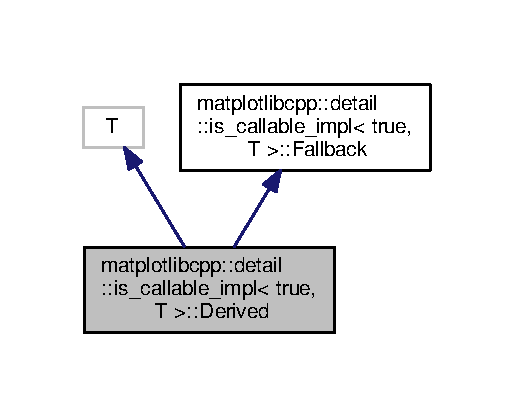
\includegraphics[width=247pt]{structmatplotlibcpp_1_1detail_1_1is__callable__impl_3_01true_00_01T_01_4_1_1Derived__inherit__graph}
\end{center}
\end{figure}


Collaboration diagram for matplotlibcpp\+:\+:detail\+:\+:is\+\_\+callable\+\_\+impl$<$ true, T $>$\+:\+:Derived\+:
\nopagebreak
\begin{figure}[H]
\begin{center}
\leavevmode
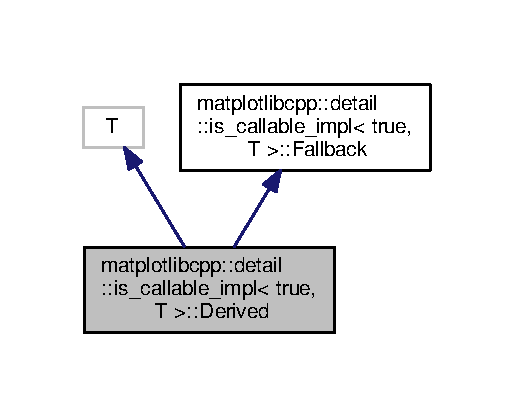
\includegraphics[width=247pt]{structmatplotlibcpp_1_1detail_1_1is__callable__impl_3_01true_00_01T_01_4_1_1Derived__coll__graph}
\end{center}
\end{figure}
\subsection*{Additional Inherited Members}


The documentation for this struct was generated from the following file\+:\begin{DoxyCompactItemize}
\item 
include/matplotlibcpp.\+h\end{DoxyCompactItemize}

\hypertarget{structmatplotlibcpp_1_1detail_1_1is__callable__impl_3_01true_00_01T_01_4_1_1Fallback}{}\section{matplotlibcpp\+:\+:detail\+:\+:is\+\_\+callable\+\_\+impl$<$ true, T $>$\+:\+:Fallback Struct Reference}
\label{structmatplotlibcpp_1_1detail_1_1is__callable__impl_3_01true_00_01T_01_4_1_1Fallback}\index{matplotlibcpp\+::detail\+::is\+\_\+callable\+\_\+impl$<$ true, T $>$\+::\+Fallback@{matplotlibcpp\+::detail\+::is\+\_\+callable\+\_\+impl$<$ true, T $>$\+::\+Fallback}}


Inheritance diagram for matplotlibcpp\+:\+:detail\+:\+:is\+\_\+callable\+\_\+impl$<$ true, T $>$\+:\+:Fallback\+:
\nopagebreak
\begin{figure}[H]
\begin{center}
\leavevmode
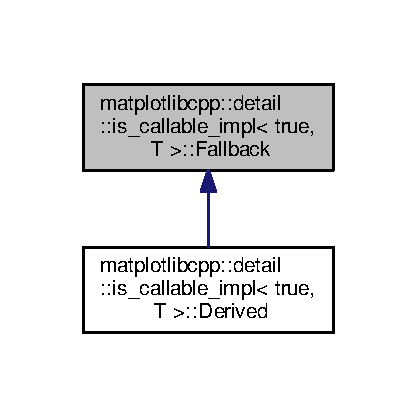
\includegraphics[width=200pt]{structmatplotlibcpp_1_1detail_1_1is__callable__impl_3_01true_00_01T_01_4_1_1Fallback__inherit__graph}
\end{center}
\end{figure}
\subsection*{Public Member Functions}
\begin{DoxyCompactItemize}
\item 
void {\bfseries operator()} ()\hypertarget{structmatplotlibcpp_1_1detail_1_1is__callable__impl_3_01true_00_01T_01_4_1_1Fallback_ad72a88facc127249a3a171a462a7a95e}{}\label{structmatplotlibcpp_1_1detail_1_1is__callable__impl_3_01true_00_01T_01_4_1_1Fallback_ad72a88facc127249a3a171a462a7a95e}

\end{DoxyCompactItemize}


The documentation for this struct was generated from the following file\+:\begin{DoxyCompactItemize}
\item 
include/matplotlibcpp.\+h\end{DoxyCompactItemize}

\hypertarget{classHuman}{}\section{Human Class Reference}
\label{classHuman}\index{Human@{Human}}
\subsection*{Public Attributes}
\begin{DoxyCompactItemize}
\item 
std\+::vector$<$ double $>$ \hyperlink{classHuman_a7978c0506328c34fdcbd883b8c5ee0cf}{centroid}\hypertarget{classHuman_a7978c0506328c34fdcbd883b8c5ee0cf}{}\label{classHuman_a7978c0506328c34fdcbd883b8c5ee0cf}

\begin{DoxyCompactList}\small\item\em The centroid of a possible human obstacle. \end{DoxyCompactList}\item 
double \hyperlink{classHuman_a27360de532f79f83fdfa810ffc1fc3db}{orientation\+Angle}\hypertarget{classHuman_a27360de532f79f83fdfa810ffc1fc3db}{}\label{classHuman_a27360de532f79f83fdfa810ffc1fc3db}

\begin{DoxyCompactList}\small\item\em The orientation angle (in radians) of a possible human obstacle. \end{DoxyCompactList}\end{DoxyCompactItemize}


The documentation for this class was generated from the following file\+:\begin{DoxyCompactItemize}
\item 
include/\hyperlink{Human_8hpp}{Human.\+hpp}\end{DoxyCompactItemize}

\hypertarget{structmatplotlibcpp_1_1detail_1_1is__callable}{}\section{matplotlibcpp\+:\+:detail\+:\+:is\+\_\+callable$<$ T $>$ Struct Template Reference}
\label{structmatplotlibcpp_1_1detail_1_1is__callable}\index{matplotlibcpp\+::detail\+::is\+\_\+callable$<$ T $>$@{matplotlibcpp\+::detail\+::is\+\_\+callable$<$ T $>$}}
\subsection*{Public Types}
\begin{DoxyCompactItemize}
\item 
typedef \hyperlink{structmatplotlibcpp_1_1detail_1_1is__callable__impl}{is\+\_\+callable\+\_\+impl}$<$ std\+::is\+\_\+class$<$ T $>$\+::value, T $>$\+::type {\bfseries type}\hypertarget{structmatplotlibcpp_1_1detail_1_1is__callable_abddc65f95805f85d5619f31cce0fbaa9}{}\label{structmatplotlibcpp_1_1detail_1_1is__callable_abddc65f95805f85d5619f31cce0fbaa9}

\end{DoxyCompactItemize}


The documentation for this struct was generated from the following file\+:\begin{DoxyCompactItemize}
\item 
include/matplotlibcpp.\+h\end{DoxyCompactItemize}

\hypertarget{structmatplotlibcpp_1_1detail_1_1is__callable__impl}{}\section{matplotlibcpp\+:\+:detail\+:\+:is\+\_\+callable\+\_\+impl$<$ obj, T $>$ Struct Template Reference}
\label{structmatplotlibcpp_1_1detail_1_1is__callable__impl}\index{matplotlibcpp\+::detail\+::is\+\_\+callable\+\_\+impl$<$ obj, T $>$@{matplotlibcpp\+::detail\+::is\+\_\+callable\+\_\+impl$<$ obj, T $>$}}


The documentation for this struct was generated from the following file\+:\begin{DoxyCompactItemize}
\item 
include/matplotlibcpp.\+h\end{DoxyCompactItemize}

\hypertarget{structmatplotlibcpp_1_1detail_1_1is__callable__impl_3_01false_00_01T_01_4}{}\section{matplotlibcpp\+:\+:detail\+:\+:is\+\_\+callable\+\_\+impl$<$ false, T $>$ Struct Template Reference}
\label{structmatplotlibcpp_1_1detail_1_1is__callable__impl_3_01false_00_01T_01_4}\index{matplotlibcpp\+::detail\+::is\+\_\+callable\+\_\+impl$<$ false, T $>$@{matplotlibcpp\+::detail\+::is\+\_\+callable\+\_\+impl$<$ false, T $>$}}
\subsection*{Public Types}
\begin{DoxyCompactItemize}
\item 
typedef is\+\_\+function$<$ T $>$ {\bfseries type}\hypertarget{structmatplotlibcpp_1_1detail_1_1is__callable__impl_3_01false_00_01T_01_4_a54b64329bf2f22cd03b8914d0bf47c3c}{}\label{structmatplotlibcpp_1_1detail_1_1is__callable__impl_3_01false_00_01T_01_4_a54b64329bf2f22cd03b8914d0bf47c3c}

\end{DoxyCompactItemize}


The documentation for this struct was generated from the following file\+:\begin{DoxyCompactItemize}
\item 
include/matplotlibcpp.\+h\end{DoxyCompactItemize}

\hypertarget{structmatplotlibcpp_1_1detail_1_1is__callable__impl_3_01true_00_01T_01_4}{}\section{matplotlibcpp\+:\+:detail\+:\+:is\+\_\+callable\+\_\+impl$<$ true, T $>$ Struct Template Reference}
\label{structmatplotlibcpp_1_1detail_1_1is__callable__impl_3_01true_00_01T_01_4}\index{matplotlibcpp\+::detail\+::is\+\_\+callable\+\_\+impl$<$ true, T $>$@{matplotlibcpp\+::detail\+::is\+\_\+callable\+\_\+impl$<$ true, T $>$}}
\subsection*{Classes}
\begin{DoxyCompactItemize}
\item 
struct \hyperlink{structmatplotlibcpp_1_1detail_1_1is__callable__impl_3_01true_00_01T_01_4_1_1Check}{Check}
\item 
struct \hyperlink{structmatplotlibcpp_1_1detail_1_1is__callable__impl_3_01true_00_01T_01_4_1_1Derived}{Derived}
\item 
struct \hyperlink{structmatplotlibcpp_1_1detail_1_1is__callable__impl_3_01true_00_01T_01_4_1_1Fallback}{Fallback}
\end{DoxyCompactItemize}
\subsection*{Static Public Member Functions}
\begin{DoxyCompactItemize}
\item 
{\footnotesize template$<$typename U $>$ }\\static std\+::true\+\_\+type {\bfseries test} (...)\hypertarget{structmatplotlibcpp_1_1detail_1_1is__callable__impl_3_01true_00_01T_01_4_a0a9fd9d26d8d3cb932a4186a17a54026}{}\label{structmatplotlibcpp_1_1detail_1_1is__callable__impl_3_01true_00_01T_01_4_a0a9fd9d26d8d3cb932a4186a17a54026}

\item 
{\footnotesize template$<$typename U $>$ }\\static std\+::false\+\_\+type {\bfseries test} (Check$<$ void(Fallback\+::$\ast$)(),\&U\+::operator()$>$$\ast$)\hypertarget{structmatplotlibcpp_1_1detail_1_1is__callable__impl_3_01true_00_01T_01_4_abf810ecef316f35db92e472508f643ce}{}\label{structmatplotlibcpp_1_1detail_1_1is__callable__impl_3_01true_00_01T_01_4_abf810ecef316f35db92e472508f643ce}

\end{DoxyCompactItemize}
\subsection*{Public Attributes}
\begin{DoxyCompactItemize}
\item 
decltype(test$<$ Derived $>$(nullptr)) typedef {\bfseries type}\hypertarget{structmatplotlibcpp_1_1detail_1_1is__callable__impl_3_01true_00_01T_01_4_ab3b84ab99dcdc4a7de6497c5b0985216}{}\label{structmatplotlibcpp_1_1detail_1_1is__callable__impl_3_01true_00_01T_01_4_ab3b84ab99dcdc4a7de6497c5b0985216}

\item 
decltype(\&Fallback\+::operator()) typedef {\bfseries dtype}\hypertarget{structmatplotlibcpp_1_1detail_1_1is__callable__impl_3_01true_00_01T_01_4_aedc864521ba0dc4e9e01eb1d8a32bcbc}{}\label{structmatplotlibcpp_1_1detail_1_1is__callable__impl_3_01true_00_01T_01_4_aedc864521ba0dc4e9e01eb1d8a32bcbc}

\end{DoxyCompactItemize}
\subsection*{Static Public Attributes}
\begin{DoxyCompactItemize}
\item 
static constexpr bool {\bfseries value} = type\+::value\hypertarget{structmatplotlibcpp_1_1detail_1_1is__callable__impl_3_01true_00_01T_01_4_a254367a81240c8cfc1c281043210076f}{}\label{structmatplotlibcpp_1_1detail_1_1is__callable__impl_3_01true_00_01T_01_4_a254367a81240c8cfc1c281043210076f}

\end{DoxyCompactItemize}


The documentation for this struct was generated from the following file\+:\begin{DoxyCompactItemize}
\item 
include/matplotlibcpp.\+h\end{DoxyCompactItemize}

\hypertarget{classObstacle}{}\section{Obstacle Class Reference}
\label{classObstacle}\index{Obstacle@{Obstacle}}
\subsection*{Public Attributes}
\begin{DoxyCompactItemize}
\item 
std\+::vector$<$ double $>$ \hyperlink{classObstacle_a50648250ad46b7c02858dd34ad705b82}{left\+Most\+Point}\hypertarget{classObstacle_a50648250ad46b7c02858dd34ad705b82}{}\label{classObstacle_a50648250ad46b7c02858dd34ad705b82}

\begin{DoxyCompactList}\small\item\em The left most point in the obstacle cluster. \end{DoxyCompactList}\item 
std\+::vector$<$ double $>$ \hyperlink{classObstacle_a98d92d6458a8bd9c974b0d4eb0a23f6a}{right\+Most\+Point}\hypertarget{classObstacle_a98d92d6458a8bd9c974b0d4eb0a23f6a}{}\label{classObstacle_a98d92d6458a8bd9c974b0d4eb0a23f6a}

\begin{DoxyCompactList}\small\item\em The right most point in the obstacle cluster. \end{DoxyCompactList}\item 
std\+::vector$<$ double $>$ \hyperlink{classObstacle_a19b8541b4cb1afdd6041a6cbffc12fb4}{mid\+Point}\hypertarget{classObstacle_a19b8541b4cb1afdd6041a6cbffc12fb4}{}\label{classObstacle_a19b8541b4cb1afdd6041a6cbffc12fb4}

\begin{DoxyCompactList}\small\item\em The midpoint in the obstacle cluster. \end{DoxyCompactList}\item 
double \hyperlink{classObstacle_a72ad3fd5d33750946ffcd5497ad96449}{largest\+Grad}\hypertarget{classObstacle_a72ad3fd5d33750946ffcd5497ad96449}{}\label{classObstacle_a72ad3fd5d33750946ffcd5497ad96449}

\begin{DoxyCompactList}\small\item\em The largest gradient in the obstacle cluster. \end{DoxyCompactList}\item 
double \hyperlink{classObstacle_a8be12479fb083dec515e4405fd1853b1}{smallest\+Grad}\hypertarget{classObstacle_a8be12479fb083dec515e4405fd1853b1}{}\label{classObstacle_a8be12479fb083dec515e4405fd1853b1}

\begin{DoxyCompactList}\small\item\em The smallest gradient in the obstacle cluster. \end{DoxyCompactList}\end{DoxyCompactItemize}


The documentation for this class was generated from the following file\+:\begin{DoxyCompactItemize}
\item 
include/\hyperlink{Obstacle_8hpp}{Obstacle.\+hpp}\end{DoxyCompactItemize}

\hypertarget{classmatplotlibcpp_1_1Plot}{}\section{matplotlibcpp\+:\+:Plot Class Reference}
\label{classmatplotlibcpp_1_1Plot}\index{matplotlibcpp\+::\+Plot@{matplotlibcpp\+::\+Plot}}
\subsection*{Public Member Functions}
\begin{DoxyCompactItemize}
\item 
{\footnotesize template$<$typename Numeric $>$ }\\{\bfseries Plot} (const std\+::string \&name, const std\+::vector$<$ Numeric $>$ \&x, const std\+::vector$<$ Numeric $>$ \&y, const std\+::string \&format=\char`\"{}\char`\"{})\hypertarget{classmatplotlibcpp_1_1Plot_a6ab809f4fc44d6e4eadb100cba5b519e}{}\label{classmatplotlibcpp_1_1Plot_a6ab809f4fc44d6e4eadb100cba5b519e}

\item 
{\bfseries Plot} (const std\+::string \&name=\char`\"{}\char`\"{}, const std\+::string \&format=\char`\"{}\char`\"{})\hypertarget{classmatplotlibcpp_1_1Plot_ab24b1e66f705495fda89621df753ed0b}{}\label{classmatplotlibcpp_1_1Plot_ab24b1e66f705495fda89621df753ed0b}

\item 
{\footnotesize template$<$typename Numeric $>$ }\\bool {\bfseries update} (const std\+::vector$<$ Numeric $>$ \&x, const std\+::vector$<$ Numeric $>$ \&y)\hypertarget{classmatplotlibcpp_1_1Plot_ac515760537365754e3437322e87cfc79}{}\label{classmatplotlibcpp_1_1Plot_ac515760537365754e3437322e87cfc79}

\item 
bool {\bfseries clear} ()\hypertarget{classmatplotlibcpp_1_1Plot_a177f13fea5b50e991a373bdbea36fb59}{}\label{classmatplotlibcpp_1_1Plot_a177f13fea5b50e991a373bdbea36fb59}

\item 
void {\bfseries remove} ()\hypertarget{classmatplotlibcpp_1_1Plot_ac78c9ebb89d13558046ea23eee188aea}{}\label{classmatplotlibcpp_1_1Plot_ac78c9ebb89d13558046ea23eee188aea}

\end{DoxyCompactItemize}


The documentation for this class was generated from the following file\+:\begin{DoxyCompactItemize}
\item 
include/matplotlibcpp.\+h\end{DoxyCompactItemize}

\hypertarget{structmatplotlibcpp_1_1detail_1_1plot__impl}{}\section{matplotlibcpp\+:\+:detail\+:\+:plot\+\_\+impl$<$ Is\+Y\+Data\+Callable $>$ Struct Template Reference}
\label{structmatplotlibcpp_1_1detail_1_1plot__impl}\index{matplotlibcpp\+::detail\+::plot\+\_\+impl$<$ Is\+Y\+Data\+Callable $>$@{matplotlibcpp\+::detail\+::plot\+\_\+impl$<$ Is\+Y\+Data\+Callable $>$}}


The documentation for this struct was generated from the following file\+:\begin{DoxyCompactItemize}
\item 
include/matplotlibcpp.\+h\end{DoxyCompactItemize}

\hypertarget{structmatplotlibcpp_1_1detail_1_1plot__impl_3_01std_1_1false__type_01_4}{}\section{matplotlibcpp\+:\+:detail\+:\+:plot\+\_\+impl$<$ std\+:\+:false\+\_\+type $>$ Struct Template Reference}
\label{structmatplotlibcpp_1_1detail_1_1plot__impl_3_01std_1_1false__type_01_4}\index{matplotlibcpp\+::detail\+::plot\+\_\+impl$<$ std\+::false\+\_\+type $>$@{matplotlibcpp\+::detail\+::plot\+\_\+impl$<$ std\+::false\+\_\+type $>$}}
\subsection*{Public Member Functions}
\begin{DoxyCompactItemize}
\item 
{\footnotesize template$<$typename IterableX , typename IterableY $>$ }\\bool {\bfseries operator()} (const IterableX \&x, const IterableY \&y, const std\+::string \&format)\hypertarget{structmatplotlibcpp_1_1detail_1_1plot__impl_3_01std_1_1false__type_01_4_ab430540b63185e4a76526b47d3b195e5}{}\label{structmatplotlibcpp_1_1detail_1_1plot__impl_3_01std_1_1false__type_01_4_ab430540b63185e4a76526b47d3b195e5}

\end{DoxyCompactItemize}


The documentation for this struct was generated from the following file\+:\begin{DoxyCompactItemize}
\item 
include/matplotlibcpp.\+h\end{DoxyCompactItemize}

\hypertarget{structmatplotlibcpp_1_1detail_1_1plot__impl_3_01std_1_1true__type_01_4}{}\section{matplotlibcpp\+:\+:detail\+:\+:plot\+\_\+impl$<$ std\+:\+:true\+\_\+type $>$ Struct Template Reference}
\label{structmatplotlibcpp_1_1detail_1_1plot__impl_3_01std_1_1true__type_01_4}\index{matplotlibcpp\+::detail\+::plot\+\_\+impl$<$ std\+::true\+\_\+type $>$@{matplotlibcpp\+::detail\+::plot\+\_\+impl$<$ std\+::true\+\_\+type $>$}}
\subsection*{Public Member Functions}
\begin{DoxyCompactItemize}
\item 
{\footnotesize template$<$typename Iterable , typename Callable $>$ }\\bool {\bfseries operator()} (const Iterable \&ticks, const Callable \&f, const std\+::string \&format)\hypertarget{structmatplotlibcpp_1_1detail_1_1plot__impl_3_01std_1_1true__type_01_4_ad182cd7d9a599f3a12d3ac7316b68ecb}{}\label{structmatplotlibcpp_1_1detail_1_1plot__impl_3_01std_1_1true__type_01_4_ad182cd7d9a599f3a12d3ac7316b68ecb}

\end{DoxyCompactItemize}


The documentation for this struct was generated from the following file\+:\begin{DoxyCompactItemize}
\item 
include/matplotlibcpp.\+h\end{DoxyCompactItemize}

\hypertarget{structmatplotlibcpp_1_1select__npy__type}{}\section{matplotlibcpp\+:\+:select\+\_\+npy\+\_\+type$<$ T $>$ Struct Template Reference}
\label{structmatplotlibcpp_1_1select__npy__type}\index{matplotlibcpp\+::select\+\_\+npy\+\_\+type$<$ T $>$@{matplotlibcpp\+::select\+\_\+npy\+\_\+type$<$ T $>$}}
\subsection*{Static Public Attributes}
\begin{DoxyCompactItemize}
\item 
static const N\+P\+Y\+\_\+\+T\+Y\+P\+ES {\bfseries type} = N\+P\+Y\+\_\+\+N\+O\+T\+Y\+PE\hypertarget{structmatplotlibcpp_1_1select__npy__type_acbffa4e6e1d047b52e12330446816c9c}{}\label{structmatplotlibcpp_1_1select__npy__type_acbffa4e6e1d047b52e12330446816c9c}

\end{DoxyCompactItemize}


The documentation for this struct was generated from the following file\+:\begin{DoxyCompactItemize}
\item 
include/matplotlibcpp.\+h\end{DoxyCompactItemize}

\hypertarget{structmatplotlibcpp_1_1select__npy__type_3_01bool_01_4}{}\section{matplotlibcpp\+:\+:select\+\_\+npy\+\_\+type$<$ bool $>$ Struct Template Reference}
\label{structmatplotlibcpp_1_1select__npy__type_3_01bool_01_4}\index{matplotlibcpp\+::select\+\_\+npy\+\_\+type$<$ bool $>$@{matplotlibcpp\+::select\+\_\+npy\+\_\+type$<$ bool $>$}}
\subsection*{Static Public Attributes}
\begin{DoxyCompactItemize}
\item 
static const N\+P\+Y\+\_\+\+T\+Y\+P\+ES {\bfseries type} = N\+P\+Y\+\_\+\+B\+O\+OL\hypertarget{structmatplotlibcpp_1_1select__npy__type_3_01bool_01_4_a79dc3db61a3b0f4796a29d067d5dd374}{}\label{structmatplotlibcpp_1_1select__npy__type_3_01bool_01_4_a79dc3db61a3b0f4796a29d067d5dd374}

\end{DoxyCompactItemize}


The documentation for this struct was generated from the following file\+:\begin{DoxyCompactItemize}
\item 
include/matplotlibcpp.\+h\end{DoxyCompactItemize}

\hypertarget{structmatplotlibcpp_1_1select__npy__type_3_01double_01_4}{}\section{matplotlibcpp\+:\+:select\+\_\+npy\+\_\+type$<$ double $>$ Struct Template Reference}
\label{structmatplotlibcpp_1_1select__npy__type_3_01double_01_4}\index{matplotlibcpp\+::select\+\_\+npy\+\_\+type$<$ double $>$@{matplotlibcpp\+::select\+\_\+npy\+\_\+type$<$ double $>$}}
\subsection*{Static Public Attributes}
\begin{DoxyCompactItemize}
\item 
static const N\+P\+Y\+\_\+\+T\+Y\+P\+ES {\bfseries type} = N\+P\+Y\+\_\+\+D\+O\+U\+B\+LE\hypertarget{structmatplotlibcpp_1_1select__npy__type_3_01double_01_4_a939edaf81fedb879c8c90ad13c98a709}{}\label{structmatplotlibcpp_1_1select__npy__type_3_01double_01_4_a939edaf81fedb879c8c90ad13c98a709}

\end{DoxyCompactItemize}


The documentation for this struct was generated from the following file\+:\begin{DoxyCompactItemize}
\item 
include/matplotlibcpp.\+h\end{DoxyCompactItemize}

\hypertarget{structmatplotlibcpp_1_1select__npy__type_3_01float_01_4}{}\section{matplotlibcpp\+:\+:select\+\_\+npy\+\_\+type$<$ float $>$ Struct Template Reference}
\label{structmatplotlibcpp_1_1select__npy__type_3_01float_01_4}\index{matplotlibcpp\+::select\+\_\+npy\+\_\+type$<$ float $>$@{matplotlibcpp\+::select\+\_\+npy\+\_\+type$<$ float $>$}}
\subsection*{Static Public Attributes}
\begin{DoxyCompactItemize}
\item 
static const N\+P\+Y\+\_\+\+T\+Y\+P\+ES {\bfseries type} = N\+P\+Y\+\_\+\+F\+L\+O\+AT\hypertarget{structmatplotlibcpp_1_1select__npy__type_3_01float_01_4_a7bca025a3f0cb143e566e0f575bf7f6b}{}\label{structmatplotlibcpp_1_1select__npy__type_3_01float_01_4_a7bca025a3f0cb143e566e0f575bf7f6b}

\end{DoxyCompactItemize}


The documentation for this struct was generated from the following file\+:\begin{DoxyCompactItemize}
\item 
include/matplotlibcpp.\+h\end{DoxyCompactItemize}

\hypertarget{structmatplotlibcpp_1_1select__npy__type_3_01int16__t_01_4}{}\section{matplotlibcpp\+:\+:select\+\_\+npy\+\_\+type$<$ int16\+\_\+t $>$ Struct Template Reference}
\label{structmatplotlibcpp_1_1select__npy__type_3_01int16__t_01_4}\index{matplotlibcpp\+::select\+\_\+npy\+\_\+type$<$ int16\+\_\+t $>$@{matplotlibcpp\+::select\+\_\+npy\+\_\+type$<$ int16\+\_\+t $>$}}
\subsection*{Static Public Attributes}
\begin{DoxyCompactItemize}
\item 
static const N\+P\+Y\+\_\+\+T\+Y\+P\+ES {\bfseries type} = N\+P\+Y\+\_\+\+S\+H\+O\+RT\hypertarget{structmatplotlibcpp_1_1select__npy__type_3_01int16__t_01_4_aa7e1803c594ccc58c2cd4c8818d5a158}{}\label{structmatplotlibcpp_1_1select__npy__type_3_01int16__t_01_4_aa7e1803c594ccc58c2cd4c8818d5a158}

\end{DoxyCompactItemize}


The documentation for this struct was generated from the following file\+:\begin{DoxyCompactItemize}
\item 
include/matplotlibcpp.\+h\end{DoxyCompactItemize}

\hypertarget{structmatplotlibcpp_1_1select__npy__type_3_01int32__t_01_4}{}\section{matplotlibcpp\+:\+:select\+\_\+npy\+\_\+type$<$ int32\+\_\+t $>$ Struct Template Reference}
\label{structmatplotlibcpp_1_1select__npy__type_3_01int32__t_01_4}\index{matplotlibcpp\+::select\+\_\+npy\+\_\+type$<$ int32\+\_\+t $>$@{matplotlibcpp\+::select\+\_\+npy\+\_\+type$<$ int32\+\_\+t $>$}}
\subsection*{Static Public Attributes}
\begin{DoxyCompactItemize}
\item 
static const N\+P\+Y\+\_\+\+T\+Y\+P\+ES {\bfseries type} = N\+P\+Y\+\_\+\+I\+NT\hypertarget{structmatplotlibcpp_1_1select__npy__type_3_01int32__t_01_4_abcfd0c3dc5d5e92575c04747315cb4d5}{}\label{structmatplotlibcpp_1_1select__npy__type_3_01int32__t_01_4_abcfd0c3dc5d5e92575c04747315cb4d5}

\end{DoxyCompactItemize}


The documentation for this struct was generated from the following file\+:\begin{DoxyCompactItemize}
\item 
include/matplotlibcpp.\+h\end{DoxyCompactItemize}

\hypertarget{structmatplotlibcpp_1_1select__npy__type_3_01int64__t_01_4}{}\section{matplotlibcpp\+:\+:select\+\_\+npy\+\_\+type$<$ int64\+\_\+t $>$ Struct Template Reference}
\label{structmatplotlibcpp_1_1select__npy__type_3_01int64__t_01_4}\index{matplotlibcpp\+::select\+\_\+npy\+\_\+type$<$ int64\+\_\+t $>$@{matplotlibcpp\+::select\+\_\+npy\+\_\+type$<$ int64\+\_\+t $>$}}
\subsection*{Static Public Attributes}
\begin{DoxyCompactItemize}
\item 
static const N\+P\+Y\+\_\+\+T\+Y\+P\+ES {\bfseries type} = N\+P\+Y\+\_\+\+I\+N\+T64\hypertarget{structmatplotlibcpp_1_1select__npy__type_3_01int64__t_01_4_a0d20ea35e520ad9381aca3c173f3f02d}{}\label{structmatplotlibcpp_1_1select__npy__type_3_01int64__t_01_4_a0d20ea35e520ad9381aca3c173f3f02d}

\end{DoxyCompactItemize}


The documentation for this struct was generated from the following file\+:\begin{DoxyCompactItemize}
\item 
include/matplotlibcpp.\+h\end{DoxyCompactItemize}

\hypertarget{structmatplotlibcpp_1_1select__npy__type_3_01int8__t_01_4}{}\section{matplotlibcpp\+:\+:select\+\_\+npy\+\_\+type$<$ int8\+\_\+t $>$ Struct Template Reference}
\label{structmatplotlibcpp_1_1select__npy__type_3_01int8__t_01_4}\index{matplotlibcpp\+::select\+\_\+npy\+\_\+type$<$ int8\+\_\+t $>$@{matplotlibcpp\+::select\+\_\+npy\+\_\+type$<$ int8\+\_\+t $>$}}
\subsection*{Static Public Attributes}
\begin{DoxyCompactItemize}
\item 
static const N\+P\+Y\+\_\+\+T\+Y\+P\+ES {\bfseries type} = N\+P\+Y\+\_\+\+I\+N\+T8\hypertarget{structmatplotlibcpp_1_1select__npy__type_3_01int8__t_01_4_a74836a19458ed32ca8948a4337364eae}{}\label{structmatplotlibcpp_1_1select__npy__type_3_01int8__t_01_4_a74836a19458ed32ca8948a4337364eae}

\end{DoxyCompactItemize}


The documentation for this struct was generated from the following file\+:\begin{DoxyCompactItemize}
\item 
include/matplotlibcpp.\+h\end{DoxyCompactItemize}

\hypertarget{structmatplotlibcpp_1_1select__npy__type_3_01uint16__t_01_4}{}\section{matplotlibcpp\+:\+:select\+\_\+npy\+\_\+type$<$ uint16\+\_\+t $>$ Struct Template Reference}
\label{structmatplotlibcpp_1_1select__npy__type_3_01uint16__t_01_4}\index{matplotlibcpp\+::select\+\_\+npy\+\_\+type$<$ uint16\+\_\+t $>$@{matplotlibcpp\+::select\+\_\+npy\+\_\+type$<$ uint16\+\_\+t $>$}}
\subsection*{Static Public Attributes}
\begin{DoxyCompactItemize}
\item 
static const N\+P\+Y\+\_\+\+T\+Y\+P\+ES {\bfseries type} = N\+P\+Y\+\_\+\+U\+S\+H\+O\+RT\hypertarget{structmatplotlibcpp_1_1select__npy__type_3_01uint16__t_01_4_aca209b33cc0bcaad16c01bff097a075f}{}\label{structmatplotlibcpp_1_1select__npy__type_3_01uint16__t_01_4_aca209b33cc0bcaad16c01bff097a075f}

\end{DoxyCompactItemize}


The documentation for this struct was generated from the following file\+:\begin{DoxyCompactItemize}
\item 
include/matplotlibcpp.\+h\end{DoxyCompactItemize}

\hypertarget{structmatplotlibcpp_1_1select__npy__type_3_01uint32__t_01_4}{}\section{matplotlibcpp\+:\+:select\+\_\+npy\+\_\+type$<$ uint32\+\_\+t $>$ Struct Template Reference}
\label{structmatplotlibcpp_1_1select__npy__type_3_01uint32__t_01_4}\index{matplotlibcpp\+::select\+\_\+npy\+\_\+type$<$ uint32\+\_\+t $>$@{matplotlibcpp\+::select\+\_\+npy\+\_\+type$<$ uint32\+\_\+t $>$}}
\subsection*{Static Public Attributes}
\begin{DoxyCompactItemize}
\item 
static const N\+P\+Y\+\_\+\+T\+Y\+P\+ES {\bfseries type} = N\+P\+Y\+\_\+\+U\+L\+O\+NG\hypertarget{structmatplotlibcpp_1_1select__npy__type_3_01uint32__t_01_4_a21b0fbd17b661ef512cc1c3c728dfa60}{}\label{structmatplotlibcpp_1_1select__npy__type_3_01uint32__t_01_4_a21b0fbd17b661ef512cc1c3c728dfa60}

\end{DoxyCompactItemize}


The documentation for this struct was generated from the following file\+:\begin{DoxyCompactItemize}
\item 
include/matplotlibcpp.\+h\end{DoxyCompactItemize}

\hypertarget{structmatplotlibcpp_1_1select__npy__type_3_01uint64__t_01_4}{}\section{matplotlibcpp\+:\+:select\+\_\+npy\+\_\+type$<$ uint64\+\_\+t $>$ Struct Template Reference}
\label{structmatplotlibcpp_1_1select__npy__type_3_01uint64__t_01_4}\index{matplotlibcpp\+::select\+\_\+npy\+\_\+type$<$ uint64\+\_\+t $>$@{matplotlibcpp\+::select\+\_\+npy\+\_\+type$<$ uint64\+\_\+t $>$}}
\subsection*{Static Public Attributes}
\begin{DoxyCompactItemize}
\item 
static const N\+P\+Y\+\_\+\+T\+Y\+P\+ES {\bfseries type} = N\+P\+Y\+\_\+\+U\+I\+N\+T64\hypertarget{structmatplotlibcpp_1_1select__npy__type_3_01uint64__t_01_4_a8d5871452f90ff04452f0416bee54fca}{}\label{structmatplotlibcpp_1_1select__npy__type_3_01uint64__t_01_4_a8d5871452f90ff04452f0416bee54fca}

\end{DoxyCompactItemize}


The documentation for this struct was generated from the following file\+:\begin{DoxyCompactItemize}
\item 
include/matplotlibcpp.\+h\end{DoxyCompactItemize}

\hypertarget{structmatplotlibcpp_1_1select__npy__type_3_01uint8__t_01_4}{}\section{matplotlibcpp\+:\+:select\+\_\+npy\+\_\+type$<$ uint8\+\_\+t $>$ Struct Template Reference}
\label{structmatplotlibcpp_1_1select__npy__type_3_01uint8__t_01_4}\index{matplotlibcpp\+::select\+\_\+npy\+\_\+type$<$ uint8\+\_\+t $>$@{matplotlibcpp\+::select\+\_\+npy\+\_\+type$<$ uint8\+\_\+t $>$}}
\subsection*{Static Public Attributes}
\begin{DoxyCompactItemize}
\item 
static const N\+P\+Y\+\_\+\+T\+Y\+P\+ES {\bfseries type} = N\+P\+Y\+\_\+\+U\+I\+N\+T8\hypertarget{structmatplotlibcpp_1_1select__npy__type_3_01uint8__t_01_4_a6e80bfd252a69f14ff869c8b4fbb9e54}{}\label{structmatplotlibcpp_1_1select__npy__type_3_01uint8__t_01_4_a6e80bfd252a69f14ff869c8b4fbb9e54}

\end{DoxyCompactItemize}


The documentation for this struct was generated from the following file\+:\begin{DoxyCompactItemize}
\item 
include/matplotlibcpp.\+h\end{DoxyCompactItemize}

\hypertarget{classXingyun}{}\section{Xingyun Class Reference}
\label{classXingyun}\index{Xingyun@{Xingyun}}
\subsection*{Public Member Functions}
\begin{DoxyCompactItemize}
\item 
std\+::vector$<$ \hyperlink{classHuman}{Human} $>$ \hyperlink{classXingyun_acc758f9857fc25df9e9a6a1543753d4b}{human\+Perception} (std\+::string lidar\+Dataset\+Filename)
\begin{DoxyCompactList}\small\item\em Main function to detect human. \end{DoxyCompactList}\item 
void \hyperlink{classXingyun_ae28021d0f1ecf6b320ef0bfbf9939a6c}{visualization} ()\hypertarget{classXingyun_ae28021d0f1ecf6b320ef0bfbf9939a6c}{}\label{classXingyun_ae28021d0f1ecf6b320ef0bfbf9939a6c}

\begin{DoxyCompactList}\small\item\em Show the output map. \end{DoxyCompactList}\item 
std\+::vector$<$ double $>$ \hyperlink{classXingyun_a019decd49b73c16a5632006d83d529cf}{get\+Raw\+Lidar\+Distances} ()
\begin{DoxyCompactList}\small\item\em Get raw\+Lidar\+Distances. \end{DoxyCompactList}\item 
std\+::vector$<$ std\+::vector$<$ double $>$ $>$ \hyperlink{classXingyun_a1313253c1365a2223470896892070e96}{get\+Point\+Cloud\+Polar} ()
\begin{DoxyCompactList}\small\item\em Get point\+Cloud\+Polar. \end{DoxyCompactList}\item 
std\+::vector$<$ std\+::vector$<$ double $>$ $>$ \hyperlink{classXingyun_ac26c7bf54cf60382650272b9488a32f2}{get\+Point\+Cloud\+Cartesian} ()
\begin{DoxyCompactList}\small\item\em Get point\+Cloud\+Cartesian. \end{DoxyCompactList}\item 
std\+::vector$<$ \hyperlink{classObstacle}{Obstacle} $>$ \hyperlink{classXingyun_af5631d38103c3bcc312881a940780be8}{get\+Obstacle\+List} ()
\begin{DoxyCompactList}\small\item\em Get obstacle\+List. \end{DoxyCompactList}\item 
std\+::vector$<$ \hyperlink{classObstacle}{Obstacle} $>$ \hyperlink{classXingyun_a7ede3f1d105300c62f5fa313e00dd6f3}{get\+Leg\+List} ()
\begin{DoxyCompactList}\small\item\em Get leg\+List. \end{DoxyCompactList}\item 
std\+::vector$<$ \hyperlink{classHuman}{Human} $>$ \hyperlink{classXingyun_ae50af290dc24fffd479328c91864abfa}{get\+Human\+List} ()
\begin{DoxyCompactList}\small\item\em Get human\+List. \end{DoxyCompactList}\end{DoxyCompactItemize}


\subsection{Member Function Documentation}
\index{Xingyun@{Xingyun}!get\+Human\+List@{get\+Human\+List}}
\index{get\+Human\+List@{get\+Human\+List}!Xingyun@{Xingyun}}
\subsubsection[{\texorpdfstring{get\+Human\+List()}{getHumanList()}}]{\setlength{\rightskip}{0pt plus 5cm}std\+::vector$<$ {\bf Human} $>$ Xingyun\+::get\+Human\+List (
\begin{DoxyParamCaption}
{}
\end{DoxyParamCaption}
)}\hypertarget{classXingyun_ae50af290dc24fffd479328c91864abfa}{}\label{classXingyun_ae50af290dc24fffd479328c91864abfa}


Get human\+List. 

\begin{DoxyReturn}{Returns}
human\+List -\/ List of humans. 
\end{DoxyReturn}
\index{Xingyun@{Xingyun}!get\+Leg\+List@{get\+Leg\+List}}
\index{get\+Leg\+List@{get\+Leg\+List}!Xingyun@{Xingyun}}
\subsubsection[{\texorpdfstring{get\+Leg\+List()}{getLegList()}}]{\setlength{\rightskip}{0pt plus 5cm}std\+::vector$<$ {\bf Obstacle} $>$ Xingyun\+::get\+Leg\+List (
\begin{DoxyParamCaption}
{}
\end{DoxyParamCaption}
)}\hypertarget{classXingyun_a7ede3f1d105300c62f5fa313e00dd6f3}{}\label{classXingyun_a7ede3f1d105300c62f5fa313e00dd6f3}


Get leg\+List. 

\begin{DoxyReturn}{Returns}
leg\+List -\/ List of legs. 
\end{DoxyReturn}
\index{Xingyun@{Xingyun}!get\+Obstacle\+List@{get\+Obstacle\+List}}
\index{get\+Obstacle\+List@{get\+Obstacle\+List}!Xingyun@{Xingyun}}
\subsubsection[{\texorpdfstring{get\+Obstacle\+List()}{getObstacleList()}}]{\setlength{\rightskip}{0pt plus 5cm}std\+::vector$<$ {\bf Obstacle} $>$ Xingyun\+::get\+Obstacle\+List (
\begin{DoxyParamCaption}
{}
\end{DoxyParamCaption}
)}\hypertarget{classXingyun_af5631d38103c3bcc312881a940780be8}{}\label{classXingyun_af5631d38103c3bcc312881a940780be8}


Get obstacle\+List. 

\begin{DoxyReturn}{Returns}
obstacle\+List -\/ List of obstacles. 
\end{DoxyReturn}
\index{Xingyun@{Xingyun}!get\+Point\+Cloud\+Cartesian@{get\+Point\+Cloud\+Cartesian}}
\index{get\+Point\+Cloud\+Cartesian@{get\+Point\+Cloud\+Cartesian}!Xingyun@{Xingyun}}
\subsubsection[{\texorpdfstring{get\+Point\+Cloud\+Cartesian()}{getPointCloudCartesian()}}]{\setlength{\rightskip}{0pt plus 5cm}std\+::vector$<$ std\+::vector$<$ double $>$ $>$ Xingyun\+::get\+Point\+Cloud\+Cartesian (
\begin{DoxyParamCaption}
{}
\end{DoxyParamCaption}
)}\hypertarget{classXingyun_ac26c7bf54cf60382650272b9488a32f2}{}\label{classXingyun_ac26c7bf54cf60382650272b9488a32f2}


Get point\+Cloud\+Cartesian. 

\begin{DoxyReturn}{Returns}
point\+Cloud\+Cartesian -\/ Converted data in Cartesian coordinate. 
\end{DoxyReturn}
\index{Xingyun@{Xingyun}!get\+Point\+Cloud\+Polar@{get\+Point\+Cloud\+Polar}}
\index{get\+Point\+Cloud\+Polar@{get\+Point\+Cloud\+Polar}!Xingyun@{Xingyun}}
\subsubsection[{\texorpdfstring{get\+Point\+Cloud\+Polar()}{getPointCloudPolar()}}]{\setlength{\rightskip}{0pt plus 5cm}std\+::vector$<$ std\+::vector$<$ double $>$ $>$ Xingyun\+::get\+Point\+Cloud\+Polar (
\begin{DoxyParamCaption}
{}
\end{DoxyParamCaption}
)}\hypertarget{classXingyun_a1313253c1365a2223470896892070e96}{}\label{classXingyun_a1313253c1365a2223470896892070e96}


Get point\+Cloud\+Polar. 

\begin{DoxyReturn}{Returns}
point\+Cloud\+Polar -\/ Converted data in Polar coordinate. 
\end{DoxyReturn}
\index{Xingyun@{Xingyun}!get\+Raw\+Lidar\+Distances@{get\+Raw\+Lidar\+Distances}}
\index{get\+Raw\+Lidar\+Distances@{get\+Raw\+Lidar\+Distances}!Xingyun@{Xingyun}}
\subsubsection[{\texorpdfstring{get\+Raw\+Lidar\+Distances()}{getRawLidarDistances()}}]{\setlength{\rightskip}{0pt plus 5cm}std\+::vector$<$ double $>$ Xingyun\+::get\+Raw\+Lidar\+Distances (
\begin{DoxyParamCaption}
{}
\end{DoxyParamCaption}
)}\hypertarget{classXingyun_a019decd49b73c16a5632006d83d529cf}{}\label{classXingyun_a019decd49b73c16a5632006d83d529cf}


Get raw\+Lidar\+Distances. 

\begin{DoxyReturn}{Returns}
raw\+Lidar\+Distances -\/ Raw data. 
\end{DoxyReturn}
\index{Xingyun@{Xingyun}!human\+Perception@{human\+Perception}}
\index{human\+Perception@{human\+Perception}!Xingyun@{Xingyun}}
\subsubsection[{\texorpdfstring{human\+Perception(std\+::string lidar\+Dataset\+Filename)}{humanPerception(std::string lidarDatasetFilename)}}]{\setlength{\rightskip}{0pt plus 5cm}std\+::vector$<$ {\bf Human} $>$ Xingyun\+::human\+Perception (
\begin{DoxyParamCaption}
\item[{std\+::string}]{lidar\+Dataset\+Filename}
\end{DoxyParamCaption}
)}\hypertarget{classXingyun_acc758f9857fc25df9e9a6a1543753d4b}{}\label{classXingyun_acc758f9857fc25df9e9a6a1543753d4b}


Main function to detect human. 


\begin{DoxyParams}{Parameters}
{\em lidar\+Dataset\+Filename} & Name of the data-\/set. \\
\hline
\end{DoxyParams}
\begin{DoxyReturn}{Returns}
human\+List -\/ The detected human list.
\end{DoxyReturn}

\begin{DoxyParams}{Parameters}
{\em lidar\+Dataset\+Filename} & -\/ Name of the data-\/set. \\
\hline
\end{DoxyParams}
\begin{DoxyReturn}{Returns}
human\+List -\/ The detected human list. 
\end{DoxyReturn}


The documentation for this class was generated from the following files\+:\begin{DoxyCompactItemize}
\item 
include/\hyperlink{Xingyun_8hpp}{Xingyun.\+hpp}\item 
app/\hyperlink{Xingyun_8cpp}{Xingyun.\+cpp}\end{DoxyCompactItemize}

\chapter{File Documentation}
\hypertarget{Human_8cpp}{}\section{app/\+Human.cpp File Reference}
\label{Human_8cpp}\index{app/\+Human.\+cpp@{app/\+Human.\+cpp}}


The file \hyperlink{Human_8cpp}{Human.\+cpp} implements the \hyperlink{classHuman}{Human} class. The class will be used in \hyperlink{classXingyun}{Xingyun} class.  This project is released under the B\+S\+D-\/3-\/\+Clause License.  


{\ttfamily \#include $<$iostream$>$}\\*
{\ttfamily \#include $<$vector$>$}\\*
{\ttfamily \#include $<$Human.\+hpp$>$}\\*
Include dependency graph for Human.\+cpp\+:
\nopagebreak
\begin{figure}[H]
\begin{center}
\leavevmode
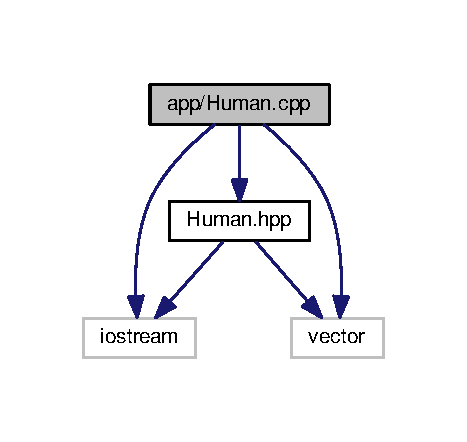
\includegraphics[width=224pt]{Human_8cpp__incl}
\end{center}
\end{figure}


\subsection{Detailed Description}
The file \hyperlink{Human_8cpp}{Human.\+cpp} implements the \hyperlink{classHuman}{Human} class. The class will be used in \hyperlink{classXingyun}{Xingyun} class.  This project is released under the B\+S\+D-\/3-\/\+Clause License. 

Copyright (c) 2019 Hao Da (Kevin) Dong, Zuyang Cao, Jing Liang

\begin{DoxyDate}{Date}
10/13/2019 
\end{DoxyDate}

\hypertarget{Obstacle_8cpp}{}\section{app/\+Obstacle.cpp File Reference}
\label{Obstacle_8cpp}\index{app/\+Obstacle.\+cpp@{app/\+Obstacle.\+cpp}}


The file \hyperlink{Obstacle_8cpp}{Obstacle.\+cpp} implements the obstacle class. The class will be used in \hyperlink{classXingyun}{Xingyun} class.  This project is released under the B\+S\+D-\/3-\/\+Clause License.  


{\ttfamily \#include $<$iostream$>$}\\*
{\ttfamily \#include $<$vector$>$}\\*
{\ttfamily \#include $<$Obstacle.\+hpp$>$}\\*
Include dependency graph for Obstacle.\+cpp\+:
\nopagebreak
\begin{figure}[H]
\begin{center}
\leavevmode
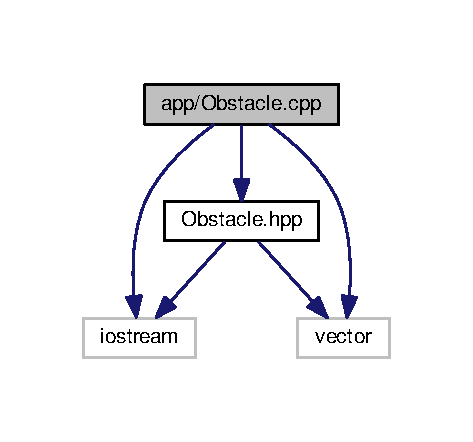
\includegraphics[width=227pt]{Obstacle_8cpp__incl}
\end{center}
\end{figure}


\subsection{Detailed Description}
The file \hyperlink{Obstacle_8cpp}{Obstacle.\+cpp} implements the obstacle class. The class will be used in \hyperlink{classXingyun}{Xingyun} class.  This project is released under the B\+S\+D-\/3-\/\+Clause License. 

Copyright (c) 2019 Hao Da (Kevin) Dong, Zuyang Cao, Jing Liang

\begin{DoxyDate}{Date}
10/13/2019 
\end{DoxyDate}

\hypertarget{Xingyun_8cpp}{}\section{app/\+Xingyun.cpp File Reference}
\label{Xingyun_8cpp}\index{app/\+Xingyun.\+cpp@{app/\+Xingyun.\+cpp}}


The file \hyperlink{Xingyun_8cpp}{Xingyun.\+cpp} implements a human perception class. The class will be used for detecting human from 2D Lidar data-\/sets.  This project is released under the B\+S\+D-\/3-\/\+Clause License.  


{\ttfamily \#include $<$matplotlibcpp.\+h$>$}\\*
{\ttfamily \#include $<$math.\+h$>$}\\*
{\ttfamily \#include $<$iostream$>$}\\*
{\ttfamily \#include $<$vector$>$}\\*
{\ttfamily \#include $<$iterator$>$}\\*
{\ttfamily \#include $<$fstream$>$}\\*
{\ttfamily \#include $<$sstream$>$}\\*
{\ttfamily \#include $<$algorithm$>$}\\*
{\ttfamily \#include $<$string$>$}\\*
{\ttfamily \#include $<$boost/range/combine.\+hpp$>$}\\*
{\ttfamily \#include $<$boost/tuple/tuple.\+hpp$>$}\\*
{\ttfamily \#include $<$boost/range/irange.\+hpp$>$}\\*
{\ttfamily \#include $<$Obstacle.\+hpp$>$}\\*
{\ttfamily \#include $<$Human.\+hpp$>$}\\*
{\ttfamily \#include $<$Xingyun.\+hpp$>$}\\*
Include dependency graph for Xingyun.\+cpp\+:
\nopagebreak
\begin{figure}[H]
\begin{center}
\leavevmode
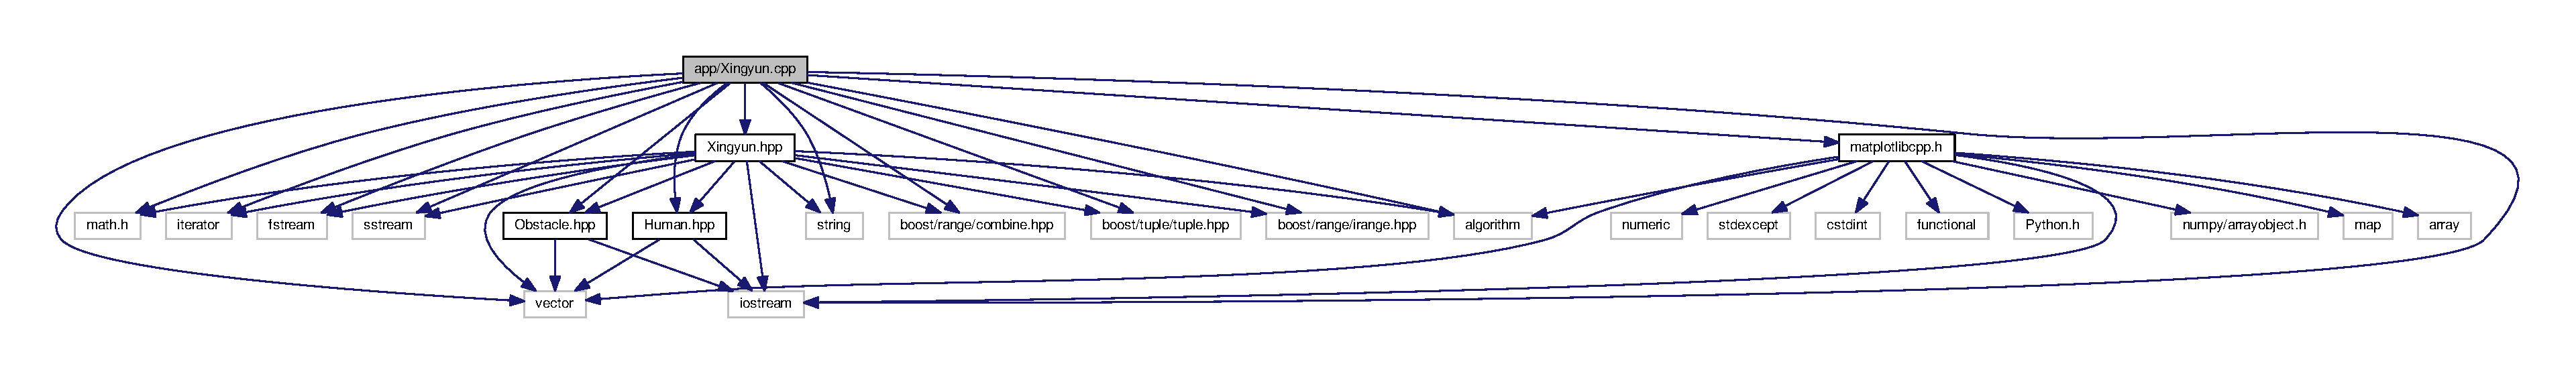
\includegraphics[width=350pt]{Xingyun_8cpp__incl}
\end{center}
\end{figure}
\subsection*{Macros}
\begin{DoxyCompactItemize}
\item 
\#define {\bfseries L\+I\+D\+A\+R\+\_\+\+R\+A\+N\+GE}~3.\+9\hypertarget{Xingyun_8cpp_a2d55d016390aaa4b7b5cb75902c0d565}{}\label{Xingyun_8cpp_a2d55d016390aaa4b7b5cb75902c0d565}

\item 
\#define {\bfseries C\+L\+U\+S\+T\+E\+R\+\_\+\+T\+H\+R\+E\+S\+H\+O\+LD}~0.\+3\hypertarget{Xingyun_8cpp_a782d9a479ed1e75611c4007d2b769178}{}\label{Xingyun_8cpp_a782d9a479ed1e75611c4007d2b769178}

\item 
\#define {\bfseries L\+E\+G\+\_\+\+D\+I\+A\+M\+E\+T\+ER}~0.\+4\hypertarget{Xingyun_8cpp_a200e7ca54e2286ed501c7b47ebfd2416}{}\label{Xingyun_8cpp_a200e7ca54e2286ed501c7b47ebfd2416}

\item 
\#define {\bfseries L\+E\+G\+\_\+\+D\+I\+S\+T\+A\+N\+CE}~0.\+3\hypertarget{Xingyun_8cpp_ad9e7e03a1e10e5c56f2d15da9e7597ab}{}\label{Xingyun_8cpp_ad9e7e03a1e10e5c56f2d15da9e7597ab}

\item 
\#define {\bfseries M\+A\+J\+O\+R\+\_\+\+A\+X\+IS}~0.\+5\hypertarget{Xingyun_8cpp_a304181058a84b4747c76a5a7828138c6}{}\label{Xingyun_8cpp_a304181058a84b4747c76a5a7828138c6}

\item 
\#define {\bfseries M\+I\+N\+O\+R\+\_\+\+A\+X\+IS}~0.\+2\hypertarget{Xingyun_8cpp_a95f1d9cc7995931e8f48bb42849e394d}{}\label{Xingyun_8cpp_a95f1d9cc7995931e8f48bb42849e394d}

\item 
\#define {\bfseries G\+R\+A\+D\+\_\+\+D\+I\+F\+F\+\_\+\+T\+H\+R\+E\+S\+H\+O\+LD}~3\hypertarget{Xingyun_8cpp_a0c4c30810e17a661ffca8be414390fc1}{}\label{Xingyun_8cpp_a0c4c30810e17a661ffca8be414390fc1}

\end{DoxyCompactItemize}


\subsection{Detailed Description}
The file \hyperlink{Xingyun_8cpp}{Xingyun.\+cpp} implements a human perception class. The class will be used for detecting human from 2D Lidar data-\/sets.  This project is released under the B\+S\+D-\/3-\/\+Clause License. 

Copyright (c) 2019 Hao Da (Kevin) Dong, Zuyang Cao, Jing Liang

\begin{DoxyDate}{Date}
10/13/2019 
\end{DoxyDate}

\hypertarget{Human_8hpp}{}\section{include/\+Human.hpp File Reference}
\label{Human_8hpp}\index{include/\+Human.\+hpp@{include/\+Human.\+hpp}}


The file \hyperlink{Human_8hpp}{Human.\+hpp} contains the header declarations for a \hyperlink{classHuman}{Human} class. The class will be used in \hyperlink{classXingyun}{Xingyun} class.  This project is released under the B\+S\+D-\/3-\/\+Clause License.  


{\ttfamily \#include $<$iostream$>$}\\*
{\ttfamily \#include $<$vector$>$}\\*
Include dependency graph for Human.\+hpp\+:
\nopagebreak
\begin{figure}[H]
\begin{center}
\leavevmode
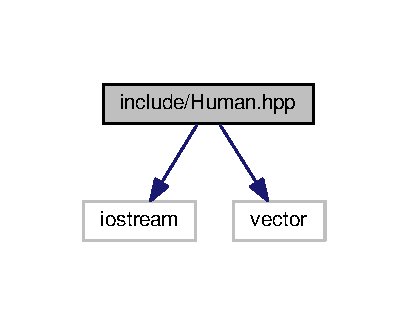
\includegraphics[width=196pt]{Human_8hpp__incl}
\end{center}
\end{figure}
This graph shows which files directly or indirectly include this file\+:
\nopagebreak
\begin{figure}[H]
\begin{center}
\leavevmode
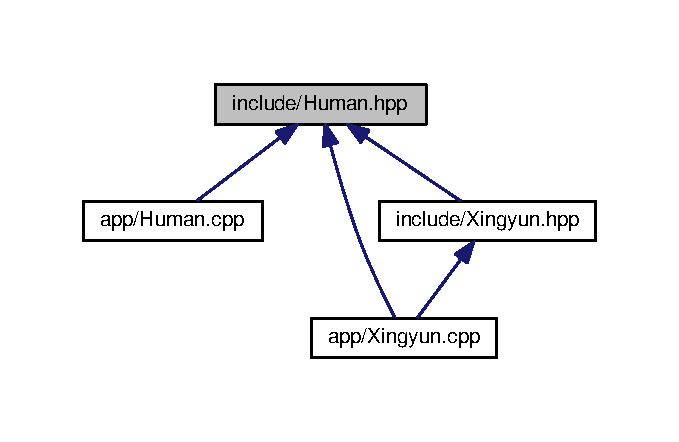
\includegraphics[width=326pt]{Human_8hpp__dep__incl}
\end{center}
\end{figure}
\subsection*{Classes}
\begin{DoxyCompactItemize}
\item 
class \hyperlink{classHuman}{Human}
\end{DoxyCompactItemize}


\subsection{Detailed Description}
The file \hyperlink{Human_8hpp}{Human.\+hpp} contains the header declarations for a \hyperlink{classHuman}{Human} class. The class will be used in \hyperlink{classXingyun}{Xingyun} class.  This project is released under the B\+S\+D-\/3-\/\+Clause License. 

Copyright (c) 2019 Hao Da (Kevin) Dong, Zuyang Cao, Jing Liang

\begin{DoxyDate}{Date}
10/13/2019 
\end{DoxyDate}

\hypertarget{Obstacle_8hpp}{}\section{include/\+Obstacle.hpp File Reference}
\label{Obstacle_8hpp}\index{include/\+Obstacle.\+hpp@{include/\+Obstacle.\+hpp}}


The file \hyperlink{Obstacle_8hpp}{Obstacle.\+hpp} contains the header declarations for a obstacle class. The class will be used in \hyperlink{classXingyun}{Xingyun} class.  This project is released under the B\+S\+D-\/3-\/\+Clause License.  


{\ttfamily \#include $<$iostream$>$}\\*
{\ttfamily \#include $<$vector$>$}\\*
Include dependency graph for Obstacle.\+hpp\+:
\nopagebreak
\begin{figure}[H]
\begin{center}
\leavevmode
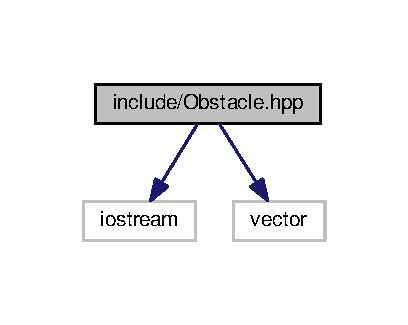
\includegraphics[width=196pt]{Obstacle_8hpp__incl}
\end{center}
\end{figure}
This graph shows which files directly or indirectly include this file\+:
\nopagebreak
\begin{figure}[H]
\begin{center}
\leavevmode
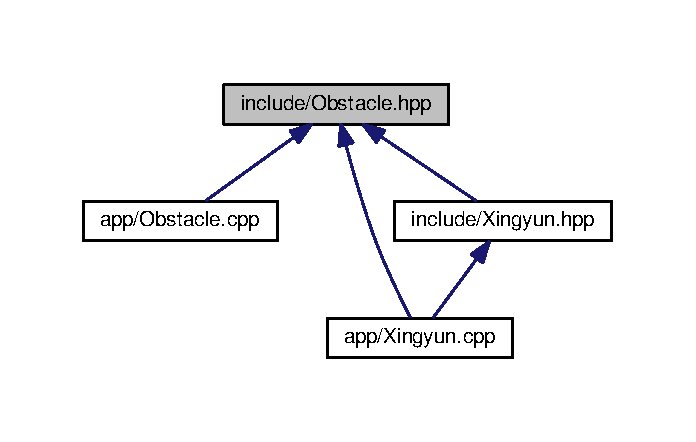
\includegraphics[width=334pt]{Obstacle_8hpp__dep__incl}
\end{center}
\end{figure}
\subsection*{Classes}
\begin{DoxyCompactItemize}
\item 
class \hyperlink{classObstacle}{Obstacle}
\end{DoxyCompactItemize}


\subsection{Detailed Description}
The file \hyperlink{Obstacle_8hpp}{Obstacle.\+hpp} contains the header declarations for a obstacle class. The class will be used in \hyperlink{classXingyun}{Xingyun} class.  This project is released under the B\+S\+D-\/3-\/\+Clause License. 

Copyright (c) 2019 Hao Da (Kevin) Dong, Zuyang Cao, Jing Liang

\begin{DoxyDate}{Date}
10/13/2019 
\end{DoxyDate}

\hypertarget{Xingyun_8hpp}{}\section{include/\+Xingyun.hpp File Reference}
\label{Xingyun_8hpp}\index{include/\+Xingyun.\+hpp@{include/\+Xingyun.\+hpp}}


The file \hyperlink{Xingyun_8hpp}{Xingyun.\+hpp} contains the header declarations for a human perception class. The class will be used for detecting human from 2D Lidar data-\/sets.  This project is released under the B\+S\+D-\/3-\/\+Clause License.  


{\ttfamily \#include $<$math.\+h$>$}\\*
{\ttfamily \#include $<$iostream$>$}\\*
{\ttfamily \#include $<$vector$>$}\\*
{\ttfamily \#include $<$iterator$>$}\\*
{\ttfamily \#include $<$fstream$>$}\\*
{\ttfamily \#include $<$sstream$>$}\\*
{\ttfamily \#include $<$algorithm$>$}\\*
{\ttfamily \#include $<$string$>$}\\*
{\ttfamily \#include $<$boost/range/combine.\+hpp$>$}\\*
{\ttfamily \#include $<$boost/tuple/tuple.\+hpp$>$}\\*
{\ttfamily \#include $<$boost/range/irange.\+hpp$>$}\\*
{\ttfamily \#include $<$Obstacle.\+hpp$>$}\\*
{\ttfamily \#include $<$Human.\+hpp$>$}\\*
Include dependency graph for Xingyun.\+hpp\+:
\nopagebreak
\begin{figure}[H]
\begin{center}
\leavevmode
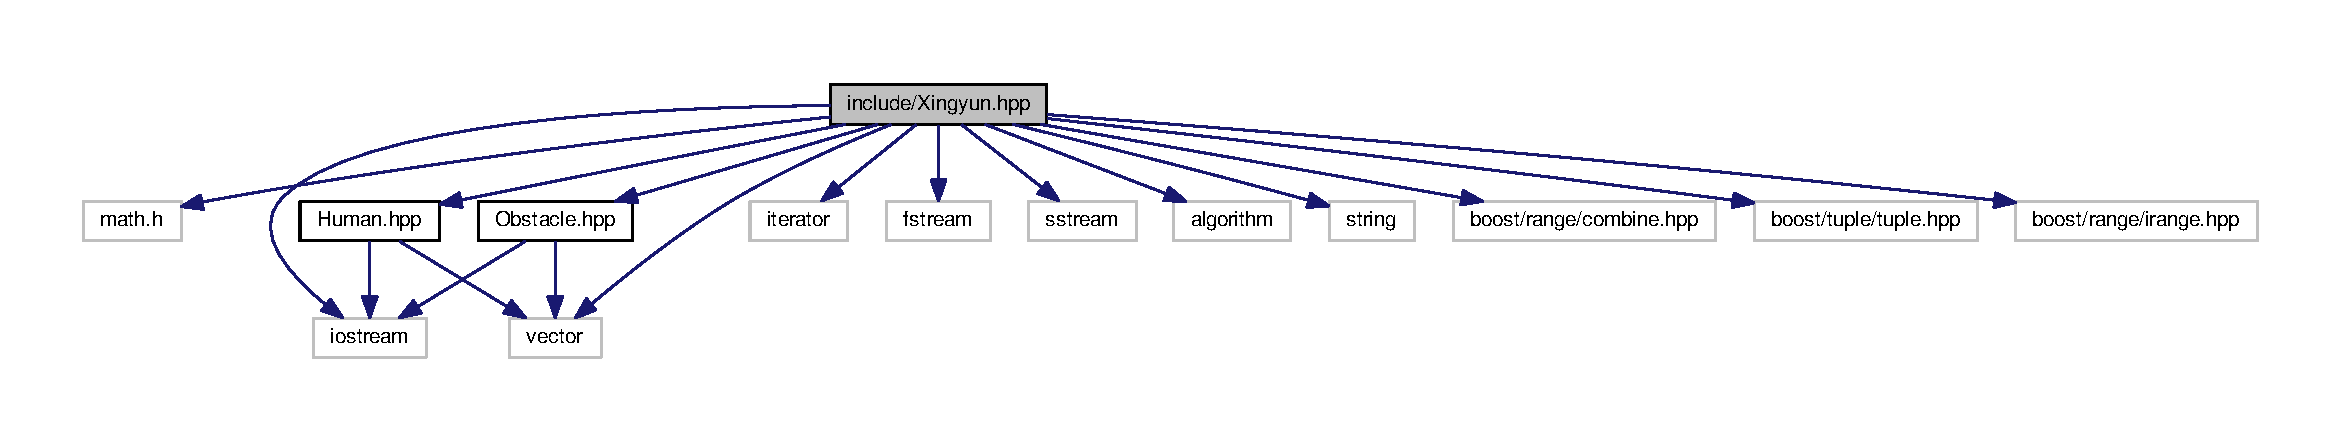
\includegraphics[width=350pt]{Xingyun_8hpp__incl}
\end{center}
\end{figure}
This graph shows which files directly or indirectly include this file\+:
\nopagebreak
\begin{figure}[H]
\begin{center}
\leavevmode
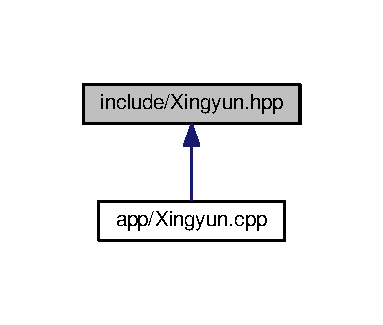
\includegraphics[width=184pt]{Xingyun_8hpp__dep__incl}
\end{center}
\end{figure}
\subsection*{Classes}
\begin{DoxyCompactItemize}
\item 
class \hyperlink{classXingyun}{Xingyun}
\end{DoxyCompactItemize}


\subsection{Detailed Description}
The file \hyperlink{Xingyun_8hpp}{Xingyun.\+hpp} contains the header declarations for a human perception class. The class will be used for detecting human from 2D Lidar data-\/sets.  This project is released under the B\+S\+D-\/3-\/\+Clause License. 

This file is to test functions of the project in scenario where person stand in front of the lidar. The file test if lidar can recognize people correct  This project is released under the B\+S\+D-\/3-\/\+Clause License.

This file is to test functions of the project in the scenario where person stand a side the lidar. The file test if lidar can recognize people correct when lidar can only detect one leg.  This project is released under the B\+S\+D-\/3-\/\+Clause License.

Copyright (c) 2019 Hao Da (Kevin) Dong, Zuyang Cao, Jing Liang

\begin{DoxyDate}{Date}
10/13/2019 
\end{DoxyDate}

%--- End generated contents ---

% Index
\backmatter
\newpage
\phantomsection
\clearemptydoublepage
\addcontentsline{toc}{chapter}{Index}
\printindex

\end{document}
